\documentclass[lang=en, hanging-titles=true]{skrapport}

\usepackage[backend=biber]{biblatex}
\addbibresource{References.bib}

\usepackage{listings}
\usepackage{listings-rust}
\usepackage[hidelinks]{hyperref}
\usepackage{graphicx} % allow embedded images
	\setkeys{Gin}{width=\linewidth,totalheight=\textheight,keepaspectratio}
	\graphicspath{{figs/papers/, figs/plots/}} % set of paths to search for images
\usepackage{svg}
	\svgpath{{figs/papers/, figs/plots/}} % not working for some reason
\usepackage{tikz}
\usepackage[11pt]{moresize}
\usepackage{subcaption}
\usepackage{afterpage}

\usepackage{ragged2e}
\usepackage[nameinlink]{cleveref}
\usepackage[nolist]{acronym}

\raggedright
\colortheme{skdoc}
\title{Title to be decided}
\author{David Kleingeld}

% % double spacing
% \linespread{1.5}

\begin{document}

\begin{titlepage}
\maketitle
\end{titlepage}
\tableofcontents
\clearpage

% constant formatting for names/concepts
\newcommand{\zookeeper}{ZooKeeper}
\newcommand{\raft}{Raft}
\newcommand{\paxos}{Paxos}
\newcommand{\multipaxos}{Multi-Paxos}
\newcommand{\ceph}{Ceph}
\newcommand{\zab}{Zab}

% inline rust code
\newcommand{\rust}{\lstinline[language=rust]}

% one day I will think of a name for this
% ideas: range fs?
\newcommand{\name}{my system}
\newcommand{\Name}{My system}
\newcommand{\graft}{Group Raft}

\newcommand{\textacro}[1]{\small{#1}}
\begin{acronym}
	\acro{mds}[\textacro{MDS}]{metadata server}
	\acro{amds}[\textacro{aMDS}]{authoratative MDS}
	\acro{cmds}[\textacro{cMDS}]{caching MDS}
	\acro{umds}[\textacro{uMDS}]{uninitialized MDS}

	\acro{hdfs}[\textacro{HDFS}]{Hadoop file system}
	\acro{pg}[\textacro{PG}]{placement group}
	\acro{crush}[\textacro{CRUSH}]{controlled, scalable, decentralized placement of replicated data}
	\acro{gfs}[\textacro{GFS}]{Google file system}
	\acro{nfs}[\textacro{NFS}]{network file system}
	\acro{osd}[\textacro{OSD}]{object store device}
	\acro{api}[\textacro{API}]{application programming interface}
	\acro{posix}[\textacro{POSIX}]{portable operation system interface}
	\acro{hpc}[\textacro{HPC}]{high performance computing}
	\acro{praft}[\textacro{pRaft}]{Presidential Raft}
	\acro{gc}[\textacro{GC}]{Garbage Collection}
	\acro{tdd}[\textacro{TDD}]{Type Driven Development}
	\acro{raii}[\textacro{RAII}]{Resource acquisition is initialization}
\end{acronym}

\definecolor{skBlue}{rgb}{0.04,0.28,0.42}
\definecolor{skRed}{rgb}{0.56,0.17,0.13}
\definecolor{skPurple}{rgb}{0.29,0.19,0.59}

\def\itsquare{\setbox0=\hbox{$\blacksquare$}%
   \pdfliteral{q 1 0 .2 1 0 0 cm}\rlap{$\blacksquare$}\pdfliteral{Q}\kern 8pt }
\def\itsquareWhite{\setbox0=\hbox{$\blacksquare$}%
   \pdfliteral{q 1 0 .2 1 0 0 cm}\rlap{$\square$}\pdfliteral{Q}\kern 8pt }

% legend box
\newcommand{\leg}[1]{\textcolor{#1}{\itsquare}}
\newcommand{\legWhite}[1]{\textcolor{#1}{\itsquareWhite}}
\newcommand{\clientLeg}{\leg{skPurple!30}}
\newcommand{\presidentLeg}{\leg{skRed!30}}
\newcommand{\amdsLeg}{\leg{skBlue!30}}
\newcommand{\cmdsLeg}{\legWhite{gray!80}}
\newcommand{\umdsLeg}{\leg{gray!20}}

% node styles
\tikzstyle{invisible}=[]
\tikzstyle{base}=[minimum width=0.5cm, minimum height=0.5cm, font=\footnotesize, align=center]
\tikzstyle{subdiagram}=[base, dashed, line width=1.0, draw=black!40]

\tikzstyle{client}=[base, rectangle, fill=skPurple!30]
\tikzstyle{president}=[base, rectangle, fill=skRed!30, font=\normalsize]
\tikzstyle{aMds}=[base, rectangle, align=left, fill=skBlue!30]
\tikzstyle{cMds}=[base, rectangle, align=left, fill=white]
\tikzstyle{uMds}=[base, rectangle, align=left, fill=gray!20]

% text styles
\tikzstyle{text_large}=[->, -to, thick, font=\normalsize, align=center]
\tikzstyle{text_small}=[->, -to, thick, font=\footnotesize, align=center]
\tikzstyle{dotted_line}=[->, -to, dashed, thick, font=\footnotesize, align=center]


\section{Introduction} \label{sec:intro}
%
% problem statement
%
% In distributed storage there is a balance between consensus and scalability.
%
% Tight consensus requirs orderd operations limiting parallel work.
%
% Existing solutions such as HadoopFS limit scalability using a single learder but provide fast tight consensus.
%
% Here I will develop a hybrid approach using a dedicated leaders for different file system subtrees.


\section{Background}
\textbf{TODO write tiny intro, do after introduction has been written}
Here we discuss what distributed computing is and when we use it. How faults and delays make it challenging to build simultaneously consistent and highly available systems. Then we look at consensus algorithms that solve those challenges. Finally, we discuss what a file system is and go over the most widely used distributed file systems: HDFS and Ceph.

\subsection{Distributed Computing}
When state-of-the-art hardware is no longer fast enough to run a system the option that remains is scaling out. Here then there is a choice, do you use an expansive, reliable high performance supercomputer or commodity servers connected by IP and Ethernet? This is the choice between High Performance (HPC) and Distributed Computing. With HPC faults in the hardware are rare and can be handled by restarting, simplifying software. In a distributed context faults are the norm, restarting the entire system is not an option as you would be down all the time. Resilience against faults comes at an often significant, cost to performance. Fault tolerance may limit scalability. As the scale of a system increases so does the frequency with which one of the parts fails. Even the most robust part will fail and given enough of them the system will fail frequently. Therefore, at very large scales HPC is not even an option. 

\subsection{Faults and Delays} \label{sec:faults}
Before we can build a fault resistant system we need to know what we can rely on. While hardware failures are the norm in distributed computing, faults are not the only issue to keep in mind. 

It is entirely normal for the clock of a computer to run slightly to fast or to slow. The resulting drift will normally be tens of milliseconds~\cite{time} unless special measures are taken\footnote{One could synchronize the time within a datacenter or provide nodes with more accurate clocks}. Event worse a process can be paused and then resumed at any time. Such a pause could be because the process thread is pre-emted, because its virtual machine is paused or because the process was paused and resumed after a while\footnote{On linux by sending SigStop then SigCont}. 

In a distributed system the computers (\textit{nodes})that form the system are connected by IP over ethernet. Ethernet gives no guarentee a packet is deliverd on time or at all. A node can be unreachable before seemingly working fine again.

Using a system model we formalize the faults that can occur. For timing there are three models. 
\begin{enumerate}
	\item The Synchronous model allowes an algorithm to assumes that clocks are synchronized within some bound and network traffic will arrive within a fixed time.
	\item The Partially synchronous model is a more realistic model. Most of the time clocks will be correct within a bound and network traffic will arrive within a fixed bound. However sometimes clocks will drift unbounded and some traffic might be delayed forever.
	\item The Asynchronous model has no clock, it is very restrictive.
\end{enumerate}

For most distributed systems we assume the Partially Synchronous model. Hardware faults cause a crash from which the node can be recoverd later. Either automatically as it restarts or after maintenance.

\section{Consensus Algorithms}
In this world where the network can not be trusted, time lies to us and servers will randomly crash and burn how can we get anything done at all? Lets discuss how we can build a system we can trust, a system that behaves \textit{consistantly}. To build such a system we need the parts that make up the system to agree with eachother, the must have \emph{Consensus}. Here I discuss three well known solutions. Before we get to that lets look at the principle that underlies them all: \emph{The truth is defined by the majority}.

\subsubsection*{Quorums}
Imagine a node hard at work processing requests from its siblings, suddently it gets pre-empted. The other nodes notice it is no longer responding and declear it dead, they dont know its threads got paused. A few seconds later the node responds again as if nothing had happend, and in truth, unless it checks the system clock, from its perspective no time has paused. Alternatively a network error might partition the system, each group of servers can reach eachoter but not the others. The nodes in the group will declear those in the other group dead and continue their work. Usually this results in data loss if the work progresses at all.

We can solve this by voting over each descision. It will be a strange vote, no node cares about the descision itself. In most implementations the nodes only checks if it regards the sender as trustwothy or alive and then vote yes. To prove liveliness the vote proposal could include a number. Voters only vote yes if the number is correct. For example if the number is the highest they have seen. If a majority votes yes the node that requested the vote can be sure its not dead or disconnected. This is the idea behind "Quorums," majorities of nodes that vote.

\subsubsection*{paxos}
The \textsc{Paxos} algorithm\cite{paxos} uses a quorum to provide concensus. It does this by chosing a value among proposals such that only that value can be read as the accepted value. Usually it is used to build a fault tolerant distributed state machine. 

In \textsc{Paxos} there are three roles: proposer, acceptor and learner. It is possible for nodes to fullfil only one or two of these roles. For the rest of this explanation assume each node fullfils all three. To reach consensus on a new value we go through two phases: prepare and accept. Once the majority of the nodes has accepted a proposal the vale of that proposal been chosen. In \textsc{Paxos} nodes keep track of the highest proposal number $n$ they have seen. Lets go through a \textsc{Paxos} iteration from the perspective of a node trying to share something, \textit{a value}.

In the first phase a new \textit{value} is proposed by our node. It sends a \textit{perpare} request to a majority of acceptors. The request contains a proposal number $n$ higher then the highest number our node has seen up till now. The number is unique to our node. Each acceptor only responds if our number $n$ is the highest it has seen. If an acceptor had already accepted one or more requests it includes the accepted proposal with the highest $n$ in its respons.

In phase two our node checks if it got a response from the majority. Our node is going to send an accept request back to those nodes. The content of the accept request depends on what our node recieved in response to its prepare request:
%
\begin{enumerate}
	\item Our node recieved a response with number $n_p$. This means an acceptor has already accepted a value. If we continued with our own value the system would have two different accepted values. Therefor the content of our accept request will be the value from proposal $n_p$.
	\item It recieved only acknowleding replies and none contained a previously accepted value. The system has not yet decided on a value. The content of our accept request will be the value or node wants to propose but with our number $n$.
\end{enumerate}
%
The acceptors accept the request if they did not yet recieve a prepare request numberd greater then $n$. On accepting a request an acceptor sends a message to all learners\footnote{remember usually every node is a learner}. This way the learners learn a new value as soon as its ready.

% Lets get a feeling why this works by looking at what happens during network failure. Imagine the case where an accept with value $v_a$ is send to the majority $m$. The network fails and only $m-1$ nodes accept. Now 50\% of the nodes will reply $v_a$ as chosen value to learners. Any majority response to a propose request will include a node from $m-1$, thus with the accepted value. No accept request with another value then $v_a$ can therefore be send. Another value $v_b$ will thus never be accepted.

Lets get a feeling why this works by looking at what happens during node failure. Imagine a case where a minimal majority $m$ accept value $v_a$. A single node in $m$ freezes after the first learners learned of the now chosen value $v_a$. After freezing $m-1$ of the nodes will reply $v_a$ as value to learners. The learners will conclude no value has been chosen given $m-1$ is not a majority\footnote{this is not yet inconsistent, \textit{Paxos} does not guarentee consistency over wether a value has been chosen}. As seen above acceptors change their value if they recieve a higher numberd accept request. If a single node changes its value to $v_b$ consensus will break since $v_a$ has already been seen as the chosen value by a learner. A new proposal that can result into higher numberd accept requests needs a majority response. A majority response will include a node from $m-1$. That node will incude $v_a$ as the accepted value. The value for the accept request changes to $v_a$. No accept request with another value then $v_a$ can thus be issued. Another value $v_b$ will therefore never be accepted. The new accept by issued to a majority changing at least one node to have accepted $v_a$. Now at least $m+1$ nodes have $v_a$ as accepted value.



Three roles proposer, acceptor and learner
Two phases, prepare and accept
 	key insight: an accepted prepare with a higher number will spread by being the awnser to new prepares
Usually build upon with an distributed state machine 
	a leader is elected and will handle all proposals
	leader recieves client requests and turns them into state machine commands
	these are proposed, when accepted they are executed (applied) to the current state
	


\subsubsection*{raft}
\subsubsection*{consensus as a service}
% zookeeper

\subsection{File System}
A file system is a tool to organize data, the files, using a directory. Data properties, or metadata, such as a files name, identifier, size, etc. are tracked using the directory interface. Typically, the directory entry only contains the file name and its unique identifier. The identifier allows the system to fetch the other metadata. The content of the data is split into blocks which are stored on stable storage such as a hard drive or SSD. The file system defines a \ac{api} to operate on it, providing methods to \textit{create}, \textit{read}, \textit{write}, \textit{seek} and \textit{truncate} files. 

A file system can add a distinction between open and closed files. The \acp{api}: \textit{read}, \textit{write} and \textit{seek} can then be restricted to open files. This enables the system to provide some consistency guarantees. For example allowing a file to be opened only if it was not already open. This can prevent a user from corrupting data by writing concurrently to overlapping ranges in a file. There is no risk to reading from files concurrently. Depending on the system reading is even safe while appending in parallel from multiple other processes\footnote{The OS can ensure append writes are serialized, this is useful for writing to a log file where each write call appends an entire log line.}. To enable such guarantees a file system can define opening a file in read-only, append-only or read-write mode. On Linux these guarantees are opt-in\footnote{See \textsl{flock}, \textsl{fcntl} or mandatory locking}. More fine-grained semantics exist, such as opening multiple non overlapping ranges of a file for writing. 


\subsection{Existing distributed file systems}

% nfs
% 	- details 
% 	- oh oh data corruption
% 		- cache 30s by default
% 		- only written upon close (loss of data)
% 	- locking since v4 (https://linux.die.net/man/2/flock)
		% https://gavv.github.io/articles/file-locks/
% 		- locking advisable on unix (https://www.kernel.org/doc/html/v5.14-rc5/filesystems/mandatory-locking.html)

% locking problamatic and badly supported easy data corruption -> unix also no mandatory locking support (use as bridge to next section which details why locking is needed in a distributed context)

\subsubsection{Network File System}
Often we want to share filesystems over a network to share files using a \textit{Network file system}. These integrate in the interface of the client. A widely supported system is \textsc{NFS}. In \textsc{NFS} a part of a local directory is exported/shared by a local \textsc{NFS}-server. Other machines can then connect and overlay part of their directory with the exported one. The NFS protocol forwards file operations from the client to the host over the network. When an operation has been applied on the host the result is traced back to the client. To increase performance the client (almost always) caches file blocks and metadata. 

In a shared envirement it is commanplace for multiple users to simultaniously access the same files. In \textsc{NFS} this can be problamatic, as meta data is cached new files can appear to other users after 30 seconds. Further more simultaneous writes can become interleaved as each write gets split into multiple network packets \cite[p. 527]{os}, writing corrupt data. Version 4 improves the semantics respecting unix advisory file locks \cite{rfc3530}. Most applications do not take advisory locks into account still risking data corruption. 

\begin{enumerate}
	\item GFS, single node so easy
	\item Hadoop FS HA, opt in consensus
	\item Ceph, subtree partitioning
\end{enumerate}

% 	- GFS, single node so easy
% 	- Hadoop FS HA, opt in consensus
% 	- Ceph, subtree partitioning


\acresetall{}
\acused{api}
\section{Design}
Here I will go over \name{}'s design and how it enables scalable consistent distributed file storage. First I will discuss the \ac{api} exposed by my system then I will present the architecture, finally I will detail some of the system behaviour using state machine diagrams. 
%
\subsection{API and Capabilities}
\Name{} is a hierarchical file system: data is stored in files which are stored in folders. Folders can contain other folders. The file system hierarchy looks like a tree where each level may have 1 to n nodes.

The \ac{posix} has allowed applications to be developed once for all complying filesystem and forms the basis of \name{}'s \ac{api}. Expanding beyond \ac{posix}, realising performance gains in the new methods, excludes existing applications from these gains. \ceph{}~\cref{sec:ceph} does this trading some usability for performance by implementing part of the \ac{posix} \ac{hpc} IO extensions~\cite{hpc_posix}. \ceph{} also trades in all consistency for files using the \ac{hpc} \ac{api}. 

A key to my approach is expanding the file system \ac{api} beyond posix. While this makes my system harder to use it gains back the consistency lost by \ceph{} while keeping its scalability. Where \name{} expands upon \ac{posix} is the addition of \textsl{open region}. A client that \textit{opens} a file \textit{region} can access to only a range of data in the file. This \ac{api} enables consistent limited \emph{parallel concurrent} writes on or combinations of reading and writing in the same file.

Like in \ceph{} in \name{} clients gain capability when they open files. These capabilities determine what a client may perform on a file. There are four capablities: \nopagebreak
%
\begin{multicols}{4} % 2 does not work, anyway this way the list is nice, tight and centerd
\begin{itemize}
	\item read
	\item read region
	\item write
	\item write region
\end{itemize}
\end{multicols}
%
A client with write capabilities may also read data. 

\begin{samepage}
An \ac{mds} tracks the capabilities for a each of its files. The \ac{mds} will not give out a capability that breaks the following condidtion:
%
\begin{itemize}
	\item Multiple clients can have capabilities on the same file as long as write capabilities have no overlap with any region.
\end{itemize}
\end{samepage}
% 
\subsection{Architecture} \label{sec:arch}
\begin{figure}
	\begin{tikzpicture}[node distance=0.5cm and 1.0cm, auto]

    \node (president) [president] {President};

	\node (a1)[aMds, below=of president]{$\text{aMDS}_1$};
    \node (a0)[aMds, left=of a1]{$\text{aMDS}_0$};
    \node (an)[aMds, right=2.5 of a1]{$\text{aMDS}_n$};

	\foreach \n\j in {0/i,1/j,n/k}
	{
		\node (c\n_1)[cMds, below=of a\n]{cMDS};
		\node (c\n_2)[cMds, below=of c\n_1]{cMDS};
		\node (c\n_\j)[cMds, below=1 of c\n_2]{$\text{cMDS}_{\j}$};
		\node at ($(c\n_2)!.5!(c\n_\j)$) {\vdots};

		\begin{pgfonlayer}{background}
			\node [fill=black!8, fit=(a\n) (c\n_\j)] {};
		\end{pgfonlayer}
	}

	\node at ($(a1)!.5!(an)$) {\ldots}; 
	\node at ($(c1_j)!.5!(cn_k)$) {\ldots}; 
	\node at ($(c1_1)!.5!(cn_1)$) {\ldots}; 
	\node at ($(c1_2)!.5!(cn_2)$) {\ldots}; 

	\node (u1)[uMds, right =1.5 of an] {uMDS};
	\node (u2)[uMds, below =0.5 of u1] {uMDS};
	\node (u3)[uMds, below =0.5 of u2] {uMDS};
	\node (u4)[uMds, below =0.5 of u3] {uMDS};
	\node (u5)[uMds, right =0.5 of u1] {uMDS};
	\node (u6)[uMds, right =0.5 of u2] {uMDS};
	\node (u7)[uMds, right =0.5 of u3] {uMDS};
	\node (u8)[right =0.5 of u4] {\ldots};

\end{tikzpicture}

	\caption{An overview of the architecture. Note there are $n$ \acf{amds} groups, each group can have a different number of \acfp{cmds}. Not all servers in a cluster are always actively used as represented by the grey \acfp{umds}}
\end{figure}

\Name{} uses hierarchical leadership, there is one president elected by all \acp{mds}. The president in turn appoints multiple \acfp{amds} then assigns each a group of \acfp{umds}. An \ac{amds} contacts its group, and promotes each member from unassigned to caching. 

The president coordinates the cluster: monitoring the population, assigning new \acp{amds} on failures, adjusting group given failures and load balances between all groups. Load balancing is done in two ways: increasing the size of a group and increasing the number of groups using dynamic subtree partitioning~\cite{ceph} (see:~\cref{sec:subtree}). To enable the president to make load balancing decisions each \ac{amds} periodically sends file innode popularity.

Metadata changes are coordinated by an \ac{amds} it serializes metadata modifying requests and ensures the changes proliferate to the group's \acp{cmds}. Changes are only completed when they are written to half of the \acp{cmds}. Additionally the \ac{amds} keeps track of file innode popularity querying its \acp{cmds} periodically.

A groups \acp{cmds} handle metadata queries: issueing read capabilities and providing information about the filesystem tree. Additionally each \ac{cmds} tracks file innode popularity to provide to the \ac{amds}. 

It is not a good idea to assign as much \acp{cmds} to groups as possible. Each extra \ac{cmds} is one more machine the \ac{amds} needs to contact for each change. The cluster might therefore keep some \acp{umds} unassigned. I will get back to this when discussing how to add a new subtree in \Cref{sec:loadb}.
%
\subsubsection*{Consensus} \label{sec:concensus} \label{sec:praft}
Consensus communication has a performance penalty and complicates system design. Not all communication is critical to data integrity or system. I use simpler protocols where possible. 

The president is elected using \raft{}. Its coordination is communicated using \raft{}'s log replication. On failure a new president is elected by all \acp{mds} using \raft{}.

Communication from the \ac{amds} to its group members uses log replication similar to \raft{}. When an \ac{amds} is appointed it gets a \raft{} term. Changes to the metadata are shared with \acp{cmds} using log replication. An \ac{amds} can fail after the change was comitted but before the client was informed of the success. The log index is shared with the client before it is committed, on \ac{amds} failure the client can check with an \ac{cmds} to see if its log entry exists\footnote{Without the log index the client can not distinquish between failure to apply the change and a new change overriding its own.}. When the \ac{amds} fails the president selects the \ac{cmds} with the highest \textsl{commit index} as the new \ac{amds}. I call this \ac{praft}.

Load reports to the president are send over normal TCP ensuring the arrive in order. An \ac{amds} that froze, was replaced and starts working again however can still send outdated reports. By including the term of the sending \ac{amds} the president detects outdated reports and discards them.
%

\subsection{Client requests}
In this section we go over all the operations of the system, while discussing four in greater detail. I also explain how most operations are simpler forms of these four. This section is split in two parts: client requests and coordination by the president.
%
For all requests a client needs to find an official (a minister or clerk) to talk to. If the request modifies the namespace, such as write, create and delete, the client needs to contact the minister. In \Cref{fig:find_aMDS} we see how this works. Since load balancing changes and minister appointments are communicated through \raft{} each cluster member knows which ministry owns a given subtree. A client can not judge whether the node it got directions from has up to date and correct information. In the rare case the directions where incorrect this means an extra jump through an irrelevant ministry before getting correct information.
%
\begin{figure}[htbp]
	\centering
	\begin{tikzpicture}

	\node (start) [client] {Contact random node};
	\node (wrong_tree) [uMds, below =of start] {\ac{mds}\\wrong subtree};
	\node (spacer) [invisible, below=of wrong_tree] {};
	\node (amds) [aMds, left=of spacer] {\ac{amds}};
	\node (right_subtree) [cMds, right=of amds] {\ac{mds}\\right subtree};

	\begin{pgfonlayer}{background}
		\node [fill=black!8, fit=(right_subtree) (amds)] {};
	\end{pgfonlayer}

	\draw[text_small] (start) to [out=270, in=90] node [] {} (wrong_tree);
	\draw[dotted_line] (start) to [out=200, in=90] node [] {} ($(amds.north)-(0.2,0)$);
	\draw[text_small] (wrong_tree) to [out=270, in=90] node [] {} ($(amds.north)+(0.2,0)$);
	\draw[dotted_line] (wrong_tree) to [out=270, in=90] node [] {} (right_subtree);
	\draw[text_small] (right_subtree) to [out=180, in=0] node [] {} (amds);

\end{tikzpicture}

	\caption{A new client~\clientLeg{} finding the responsible minister~\amdsLeg{} for a file. Its route can go through the wrong subtree~\umdsLeg{} or via the correct ministry's clerk~\cmdsLeg{}. Whenever there is a choice the dotted line indicate the less likely path.}
	\label{fig:find_aMDS}
\end{figure}
%
\subsection*{Capabilities} \label{sec:lease}
A client needing write-capability on a file contacts the minister. It in turn checks if the lease can be given out and asks its clerks to revoke outstanding read leases that conflict. A read lease conflicts when its region overlaps with the region needed for the write capability. If a clerk lost contact with a client it can not revoke the lease and has to wait till the lease expires. The process is illustrated in \Cref{fig:write}. 

If the client needs read capabilities it sends its requests to a clerk. The clerk checks against the \raft{} log if the leases would conflict with an outstanding write lease. If no conflict is found the lease is issued and the connection to the client kept active. Keeping an active connection makes it possible to revoke the lease or quickly refresh it.
%
\begin{figure}[htbp]
	\centering
	\begin{tikzpicture}[node distance=0.5cm and 1.0cm, auto]

	\node (start) [client] {start};
	\node (find_amds) [client, subdiagram, right=1.5 of start] {find Minister};
	\draw[text_large] (start) to [out=0, in=180] node [] {} (find_amds);

	\node (check_lease) [aMds, right=1.5 of find_amds] {clear conflicting leases};
	\draw[text_small] (find_amds) to [out=0, in=180] node [] {req write} (check_lease);

	\node (cmds0) [cMds, subdiagram, below left=of check_lease] {revoke overlapping\\ read leases};
	\node (cmds1) [cMds, subdiagram, below=of cmds0] {revoke overlapping\\ read leases};
	\node (cmds2) [cMds, subdiagram, below=of cmds1] {revoke overlapping\\ read leases};
	\node (cmds_in) [invisible, right=-0.1 of cmds0] {};
	\node (cmds_out) [invisible, right=-0.1 of cmds2] {};
	\node (outstanding) [aMds, subdiagram, below right=of check_lease] {revoke overlapping\\ write lease};

	\draw[text_small] (check_lease) to [out=0, in=90] node [] {needed range} (outstanding);
	\draw[text_small] (check_lease) to [out=270, in=0] node [] {needed range} (cmds_in);

	\node (issue) [aMds, below right= of cmds_out] {no conflicting leases};
	\node (end) [client, right=of issue] {got file handle};

	\draw[text_small] (cmds_out) to [out=0, in=90] node [] {} (issue);
	\draw[text_small] (issue) to [out=0, in=180] node [] {lease} (end);
	\draw[text_small] (outstanding) to [out=270, in=90] node [] {} (issue);

	\begin{pgfonlayer}{background}
		\node [fill=black!8, fit=(cmds0) (cmds2)] {};
	\end{pgfonlayer}

\end{tikzpicture}

	\caption{A client~\clientLeg{} requesting ranged write capabilities. It finds and contacts the responsible minister~\amdsLeg{}. The minister then contacts the ministry's clerks~\cmdsLeg to clear conflicting read capabilities. Meanwhile, it revokes any conflicting write leases it gave out.}
	\label{fig:write}
\end{figure}
%
\subsection*{Namespace Changes}
Most changes to the namespace need simple edits within ministries metadata table. The client sends its request to the minister. The change is performed by adding a command to the \textit{Group Raft} log (see: \Cref{sec:praft}). Before committing the change the client gets the log index for the change. If the minister goes down before acknowledging success the client verifies if the change happened using the log index.

Removing a directory spanning one or more load balanced subtrees needs a little more care. One or more ministers will have to delete their entire subtree. This requires coordination across the entire cluster. The clients remove requests is forwarded by the minster to the \textit{president}. It in turn appends \textsl{Subtree Delete} to the cluster wide log. The client receives the log index for the command to verify success even if the \textit{president} goes down. The steps the minister takes are shown in \Cref{fig:rm}. 
%
\begin{figure}[htbp]
	\centering
	\begin{tikzpicture}[node distance=0.5cm and 1.0cm, auto]
	\node (start) [invisible] {Start};
	\node (amds_del1) [aMds, right=of start] {$\text{Minister}_j$};
	\node (pres) [president, below=of amds_del1] {Subtree delete};
	\draw[text_small] (amds_del1) to [out=270, in=90] node [] {req coordination} (pres);
	\draw[text_small] (start) to [out=0, in=180] node [] {} (amds_del1);

	\node (dots_a) [invisible, below= 1 of pres] {\ldots};
	\node (amds1) [aMds, left=0.5 of dots_a] {$\text{Minister}_1$};
	\node (amds0) [aMds, left=of amds1] {$\text{Minister}_0$};
	\node (amdsj) [aMds, right=0.5 of dots_a] {$\text{Minister}_j$};
	\node (amdsn) [aMds, right=of amdsj] {$\text{Minister}_n$};
	\node at ($(amdsj)!.5!(amdsn)$) {\ldots}; 

	\node (dots_b) [invisible, below = 1of dots_a] {\ldots};
	\node (mid) at ($(dots_a)!.5!(dots_b)$) {};
	\node (line_start) [invisible, left=5 of mid] {};
	\node (line_end) [invisible, right=6 of mid] {Raft commit};
	\draw[thick, dashed] (line_start) to [out=0, in=180] node [] {} (line_end);

	\node (amds1_b) [aMds, left=0.5 of dots_b] {$\text{Minister}_1$};
	\node (amds0_b) [aMds, left=of amds1_b] {$\text{Minister}_0$};
	\node (amdsj_b) [aMds, right=0.5 of dots_b] {$\text{Minister}_j$};
	\node (amdsn_b) [aMds, right=of amdsj_b] {$\text{Minister}_n-k$};
	\node at ($(amdsj_b)!.5!(amdsn_b)$) {\ldots}; 

	\node (dots_c) [invisible, below= 1 of dots_b] {\ldots};
	\node (amds1_c) [aMds, left=0.5 of dots_c] {$\text{Minister}_1$};
	\node (amds0_c) [aMds, left=of amds1_c] {$\text{Minister}_0$};
	\node (amdsj_c) [aMds, right=0.5 of dots_c] {$\text{Minister}_j$};
	\node (amdsn_c) [aMds, right=of amdsj_c] {$\text{Minister}_n-k$};
	\node at ($(amdsj_c)!.5!(amdsn_c)$) {\ldots}; 

	\foreach \n in {0,1,j,n}
	{
		\draw[text_small, looseness=0.3] (pres) to [out=270, in=90] node [] {} (amds\n);
	}

	\draw[text_small] (amdsj_b) to [out=270, in=90] node [] {drop sub tree} (amdsj_c);

	\draw[bracket] (amdsn_b.north east) to [out=270, in=90] node [] {} (amdsn_b.south east);

	\node (umdsn_0) [uMds, right=1 of amdsn_c] {$\text{Idle}_{0}$};
	\node (umdsn_k) [uMds, right= of umdsn_0] {$\text{Idle}_{k}$};
	\node (dots_d) at ($(umdsn_0)!.5!(umdsn_k)$) {\ldots}; 

	\draw[text_small] (amdsn_b) + (1.4,0) to [out=0, in=90] node [left, below, xshift=-6pt] {demote} (dots_d);

\end{tikzpicture}

	\caption{A minister~\amdsLeg{}, here $\text{Minister}_j$, removes a directory (tree) that is load balanced between multiple ministries. The president~\presidentLeg{} coordinates the removal by appending a command to the log. Once it is committed the ministers hosting subtrees of the directory demote themselves to idle and $\text{Ministry}_j$ drops the directory from its db}
	\label{fig:rm}
\end{figure}
%
\subsection{Availability}
Ensuring file system availability is the responsibility of the \textit{president}. This includes replacing nodes that fail and load balancing. All ministers and clerks periodically send heartbeats to the president. In this design I improve scalability by moving tasks from a central authority (the president) to groups of nodes. Continuing this pattern we could let the ministers monitor their clerks. This is more complex than letting these report directly to the \textit{president}. However, even reporting directly to the president is not needed, instead I use the TCP ACK to the \textit{president}'s \raft{} heartbeat. When the \textit{president} fails to send a \raft{} heartbeat to a node it decides the node must be failing.

\subsubsection*{A failing minister}
When the president notices a minister has failed it will try to replace it. It queries the ministries clerks to find the ideal candidate for promotion. If it gets a response from less than half the ministry it can not safely replace the minister. At that point it marks the file subtree as down and may retry in the future. A successful replacement is illustrated in \Cref{fig:appoint}.

A clerk going down is handled by the president in one of two ways:
\begin{itemize}
	\item There is at least one idle node. The president assigns the idle node to the failing nodes group. 
	\item There are no idle nodes. The president, through raft, commands a clerk in the group with the lowest load to demote itself. Then the president drops the matter. The clerk wait till its read leases expire and unassigns.
\end{itemize}
%
When the groups' minister appends to the \textit{Group Raft} log it will notice the clerk misses entries and update it (see \cref{sec:raft}).

\begin{figure}[htbp]
	\centering
	\begin{tikzpicture}[node distance=0.5cm and 0.5cm, auto]

	\node (1) [text_large] {1)};
	\node (pres) [president, right=of 1] {President};
	\node (amds) [aMds, right = 1 of pres] {\ac{amds} (failing)};
	\node (c1) [cMds, right=of amds] {$\text{cMDS}_{1}$};
	\node (c2) [cMds, right=of c1] {$\text{cMDS}_{2}$};
	\node (cn) [cMds, right=of c2] {$\text{cMDS}_{n}$};
	\node at ($(c2.east)!.5!(cn.west)$) {\ldots}; 
	\begin{pgfonlayer}{background}
		\node [fill=black!8, fit=(amds) (cn)] {};
	\end{pgfonlayer}

	\draw[text_small] (amds) to [out=180, in=0] node [] {} (pres);
	\node at ($(amds.west)!.5!(pres.east)$) {X}; 

	\node (2) [text_large, below=1 of 1] {2)};
	\node (pres) [president, right=of 2] {President};

	\node (c1) [cMds, right=2 of pres] {$\text{cMDS}_{1}$};
	\node (c2) [cMds, right=of c1] {$\text{cMDS}_{2}$};
	\node (cn) [cMds, right=of c2] {$\text{cMDS}_{n}$};
	\node at ($(c2.east)!.5!(cn.west)$) {\ldots}; 
	\begin{pgfonlayer}{background}
		\node [fill=black!8, fit=(c1) (cn)] {};
	\end{pgfonlayer}

	\draw[text_small] (pres) to [out=0, in=180] node [] {request\\commit idx} (c1);
	\draw[text_small] (pres) to [out=270, in=270, looseness = 0.2]   node [left, below, xshift=20pt, yshift=3pt] {req. commit idx} (c2);
	\draw[text_small] (pres) to [out=270, in=270, looseness = 0.3]   node [below] {req. commit idx} (cn);

	\node (3) [text_large, below=1.5 of 2] {3)};
	\node (pres) [president, right=of 3] {President};

	\node (c1) [cMds, right=2 of pres] {$\text{cMDS}_{1}$};
	\node (c2) [cMds, right=of c1] {$\text{cMDS}_{2}$};
	\node (cn) [cMds, right=of c2] {$\text{cMDS}_{n}$};
	\node at ($(c2.east)!.5!(cn.west)$) {\ldots}; 
	\begin{pgfonlayer}{background}
		\node [fill=black!8, fit=(c1) (cn)] {};
	\end{pgfonlayer}

	\draw[text_small, <-] (pres) to [out=0, in=180] node [] {idx: $k$} (c1);
	\draw[text_small, <-] (pres) to [out=270, in=270, looseness = 0.2]   node [left, below, xshift=20pt, yshift=3pt] {idx: $k-1$} (c2);
	\draw[text_small, <-] (pres) to [out=270, in=270, looseness = 0.3]   node [below] {idx: $k-j$} (cn);

	\node (4) [text_large, below=1.5 of 3] {4)};
	\node (pres) [president, right=of 4] {President};

	\node (amds) [aMds, right=1.7 of pres] {$\text{aMDS}$};
	\node (c2) [cMds, right=of amds] {$\text{cMDS}_{2}$};
	\node (cn) [cMds, right=of c2] {$\text{cMDS}_{n}$};
	\node at ($(c2.east)!.5!(cn.west)$) {\ldots}; 
	\begin{pgfonlayer}{background}
		\node [fill=black!8, fit=(amds) (cn)] {};
	\end{pgfonlayer}
	\draw[text_small] (amds) to [out=180, in=0] node [above] {Tcp ack\\heartbeat} (pres);

\end{tikzpicture}

	\caption{A minister~\amdsLeg{} fails and does not send a heartbeat on time (1). The president~\presidentLeg{} requests the latest commit index (2). Node $\text{Clerk}_1$~\cmdsLeg{} has commit index $k$ which is the highest (3). The president has promoted $\text{Clerk}_1$ to minister, it has started sending heartbeats (4). Note the heartbeats send by the clerks are not shown.}
	\label{fig:appoint}
\end{figure}
%
\subsubsection*{Load balancing} \label{sec:loadb}
From the point of availability a system that is up but drowning in requests might as well be down. To prevent nodes from getting overloaded we actively balance the load between ministries, add and remove them and expand the read capacity of some. A load report contains CPU utilization for each node in the group and the popularity of each bit of metadata split into read and write. The President checks the balance for each report it receives.
%
\subparagraph*{Trade off} \label{sec:tradeoff}
There is a trade-off here: a larger ministry means more clerks for the minister to communicate changes to, slowing down writes. On the other side as the file system is split into more subtrees the chance increases a client will need to contact not one but multiple ministries. Furthermore, to create another ministry we usually have to shrink existing ministries. Growing a ministry can involve removing one to free up clerks. 
%
We can model the read and write capacity of a single group as:
\begin{align}
	r =& n_\text{c} \\
	w =& 1 - \sigma*n_\text{c}
\end{align}%
Here $n_\text{c}$ is the number of clerks in the group, and $\sigma$ the communication overhead added by an extra clerk. 

Now we can derive the number of clerks needed given a load. Since we want to have some unused capacity $\delta$. I set $\delta$ equal to the capacity with the current load subtracted. This gets us the following system of equations: 
\begin{align}
	\delta &= w - W \\
	\delta &= r - R
\end{align}%
Now solve for $n_\text{c}$, the number of clerks.
\begin{align}
	r - R &= w - W \\
	n_c - R &= \left(1 - \sigma*n_c\right) - W \\
	n_c &= \frac{R - W + 1}{1 + \sigma}
\end{align}
From this I draw two conclusions, any spare capacity for writing is at a cost of spare reading capacity. The number of clerks roughly the read load.
%
% TODO a load balancing algorithm/ rewrite this piece
%
\subparagraph*{Read balancing}
A ministry experiencing low read load relative to their capacity is shrunk. A ministries read load is low if it could lose a clerk without average clerk CPU utilization rising above 85\%. A ministry has multiple members not only for performance. The members form a \textit{Group Raft} cluster and ensure metadata is stored redundantly. This only works if a ministry has at least three members. To shrink a ministry the President issues a \raft{} message unassigning a clerk. 

A group under high relative read load has average clerk CPU utilization passing 95\%. The president then issues a \raft{} message assigning an idle node to the group if one is available. %TODO diff % why
%
\subparagraph*{Write balancing}
When the president decides a group can no longer handle the write-load it will try to split off some work to another group. If no existing group can handle the work the president will try to create a new group. If that is not possible then the 



% TODO Finish this piece

\begin{figure}[htbp]
	\centering
	\begin{tikzpicture}[node distance=0.5cm and 0.5cm, auto]
	\node (mds0) [aMds, subdiagram] {write overload};
	\node (pres) [president, subdiagram, right=1.2 of mds0] {no unassigned};
	\node (lpres) [invisible, left=2.6 of pres] {};
	\node (rpres) [circle, fill, inner sep=2pt, right=0.6 of pres] {};
	\draw[text_small] (mds0) to [out=0, in=180] node [midway] {load\\report} (pres);
	
	\node (a0)[aMds, below=of lpres]{$\text{Minister}_0$};
    \node (a1)[aMds, below=of a0]{$\text{Minister}_1$};
    \node (a2)[aMds, below=of a1]{$\text{Minister}_2$};

	\foreach \n in {0,1,2}
	{
		\node (c0) [cMds, right=of a\n] {$\text{Clerk}_0$};
		\node (c1) [cMds, right=of c0] {$\text{Clerk}_1$};
		\node (c2) [cMds, right=of c1] {$\text{Clerk}_2$};
		\node (c3_\n) [cMds, right=of c2] {$\text{Clerk}_3$};

		\begin{pgfonlayer}{background}
			\node [fill=black!8, fit=(a\n) (c3_\n)] {};
		\end{pgfonlayer}

		\draw[text_small, looseness = 0.5] (rpres.center) to [out=0, in=180] node [] {} (c3_\n);
	}
	\draw[text_small, -] (pres) to [out=0, in=180] node [xshift=20] {\raft{}(unassign)} (rpres.center);

	\node (c0_dots) [text_small, below=1.2 of a2] {\ldots};
	\node (c0)[cMds, right=0.2 of c0_dots]{$\text{Clerk}_3$};
	\node (c1_dots) [text_small, below=0.6 of c0_dots] {\ldots};
    \node (c1)[cMds, right=0.2 of c1_dots]{$\text{Clerk}_3$};
	\node (c2_dots) [text_small, below=0.6 of c1_dots] {\ldots};
    \node (c2)[cMds, right=0.2 of c2_dots]{$\text{Clerk}_3$};

	\begin{pgfonlayer}{background}
		\foreach \n in {0,1,2}
			\node [fill=black!8, fit=(c\n) (c\n_dots)] {};
	\end{pgfonlayer}

	\node (mid) at ($(a2)!.5!(c0)$) {};
	\node (line_start) [invisible, left=1.5 of mid] {};
	\node (line_end) [invisible, right=8 of mid] {Raft commit};
	\draw[thick, dashed] (line_start) to [out=0, in=180] node [] {} (line_end);

	\foreach \n in {0,1,2} 
	{
		\node (u\n) [uMds, right=of c\n] {Idle};
		\draw[text_small] (c\n) to [out=0, in=180] node [] {} (u\n);
	}

	\node (pres) [president, right=3 of u1] {President};
	\node (mds0) [subdiagram, dotted, draw=black, right=4 of u0] {queued load report};
	\draw[text_small] (mds0) to [out=270, in=0] node [] {} (pres);

	\foreach \n in {0,1,2}
	{
		\draw[text_small, font=\ssmall, color=black!50, dashed] (u\n.north east) 
			to [out=0, in=180, looseness=0.8, bend left] node [] {done} (pres);
	}
	\draw[text_small, font=\ssmall] (pres) to [out=180, in=0, looseness=0.8, bend left] 
		node [midway, above, xshift=20, yshift=-5] {\raft{}(assign)} (u0.south east);
	\draw[text_small, font=\ssmall] (pres) to [out=180, in=0, looseness=0.8, bend left] 
		node [xshift=-10] {\raft{}(assign)} (u1.south east);
	\draw[text_small, font=\ssmall] (pres) to [out=180, in=0, looseness=0.8, bend left] 
		node [] {\raft{}(assign and promote)} (u2.south east);

	\node (a0) [aMds, below=4.8 of a2] {$\text{Minister}_3$};
	\node (c0) [cMds, right=of a0] {$\text{Clerk}_0$};
	\node (c1) [cMds, right=of c0] {$\text{Clerk}_1$};
	\node (dots) [text_large, right=of c1] {\ldots};

	\begin{pgfonlayer}{background}
		\node [fill=black!8, fit=(a0) (c1)] {};
	\end{pgfonlayer}

	\node (mid) at ($(c2)!.6!(a0)$) {};
	\node (line_start) [invisible, left=1.5 of mid] {};
	\node (line_end) [invisible, right=8 of mid] {Raft commit};
	\draw[thick, dashed] (line_start) to [out=0, in=180] node [] {} (line_end);

\end{tikzpicture}

	\caption{A minister~\amdsLeg{} under too high a load, higher than all other, sends a load report to the president~\presidentLeg{}. It can not create a new ministry as there are no or not enough idle nodes~\umdsLeg{}. The president removes three clerks~\cmdsLeg{} from the ministries under the lightest read load and queues the load report. After the clerk removal is committed the load report is enqueued. }
	\label{fig:subtree}
\end{figure}


\section{Implementation}

mocking
async


\section{Results}
The current implementation, while functional, is far from optimal. There are bottlenecks which restrict performance and the system is unstable. It is not feasible to build a system as fast and as performant and stable as \ceph{} or \ac{hdfs} within the scope of a thesis. Experimenting around these limitations we can still answer the question we posed in the introduction. It being: can an architecture using ministries together with ranged based file locking offer an advantage over existing approaches.

To design experiments that work around the limitations we need to be clear on what the limitations are:

\begin{itemize}
	\item The \raft{} implementation sends only a single log entry at the time and log entries are sent each heartbeat period instead of whenever data becomes available. Effectively this imposes a rate limit on changing the systems metadata.
	\item Load balancing only replaces nodes that go down, it does not perform subtree partitioning at runtime (see:~\Cref{sec:subtree}).
	\item Sometimes nodes become unresponsive when making many requests that change metadata. They then miss heartbeats which triggers re-elections.
\end{itemize}

In \cref{sec:res_arg} we look at the \textit{ministry architecture} tracking how performance changes when we change the number of ministries. Then we look at \textit{ranged based file locking} in \cref{sec:res_range}, we compare write performance with and without locking. In each section I will detail how the experiments work around the limitations, ensuring their outcome would match an implementation without restrictions. Every benchmark was performed five times and all the results are presented. The nodes where monitored during each run and if an error occurred we repeated the entire run. When using multiple clients to create a larger load the nodes where given time to initialize and the test start was synchronized. All raw data is available at \href{https://github.com/dvdsk/Thesis}{github.com/dvdsk/Thesis}.

The benchmarks have been performed using the fifth generation distributed ASCI Supercomputer \cite{das5}. Each node has a dual eight-core Intel Xeon E5-2630 v3 cpus and 125G of ram. As networking delays are a key characteristic of the systems' performance we used Ethernet for the communication between nodes even though the hardware is equipped with InfiniBand. The Raft heartbeat duration was set to 75 milliseconds for all tests.

\subsection{Ministry Architecture} \label{sec:res_arg}
Here we test the impact of varying the number of ministries on performance. We expect to see an almost linear improvement with more ministries given optimal size and shape of the load.

As discussed live subtree partitioning is still unimplemented, we work around this by implementing static subtree partitioning. The load balancer starts by initializing a single ministry responsible for the root directory. Additional static ministries can be passed through command line parameters. For these test we let it initialize n-1 extra ministries at paths \textsl{/n}. Including the root ministry (it must always be present) there are now n ministries available for testing.

\subsubsection{List directory}
The first load we try is list directory. We perform 60 thousand list requests spread across all root directories from 30 clients concurrently. Each client sends the requests one after another as fast as possible. To keep the overhead from sending back the directory content small each directory contains only 10 files. The client processes are spread between 3 physical nodes.

The 2000 requests each client sends can be in two different orders: \textit{batch} and \textit{stride}. In \textit{batch} a client performs all the requests for a single directory before sending those for the next. When using the \textit{stride} pattern a client sends a request to the first directory and then sends the next request to another directory. There were a few extreme outliers, these where further out then 4 standard deviations. They are not shown in the plots. % TODO: change test, make batch and stride orders random such that they dont all hit ministry one first... <08-08-22> 

In \Cref{fig:ls_vs_ministries} we see a violin plot comparing the two request orders for clusters with various number of ministries. On the Y-axis we see the time it took a single request to complete. A wider distribution means more requests where completed within the same time. Note the multimodal distribution, the increasing duration for the slowest requests as the number of ministries increases and the difference in the fastest times between batch and stride.

\Cref{fig:ls_cdf} shows \acp{cdf} of clients performing 60 thousand list directory requests in \textit{batch} mode for varying amount of ministries. On the Y-axis are the proportion of requests that complete within the time on the X-axis. Note using \textit{one} ministry is always the fastest followed initially by a configuration using \textit{five} ministries until 80\% of requests complete. Past 80\% the second place it taken by the configuration with \textit{two} ministries.

\begin{figure}[bp]
	\centering
	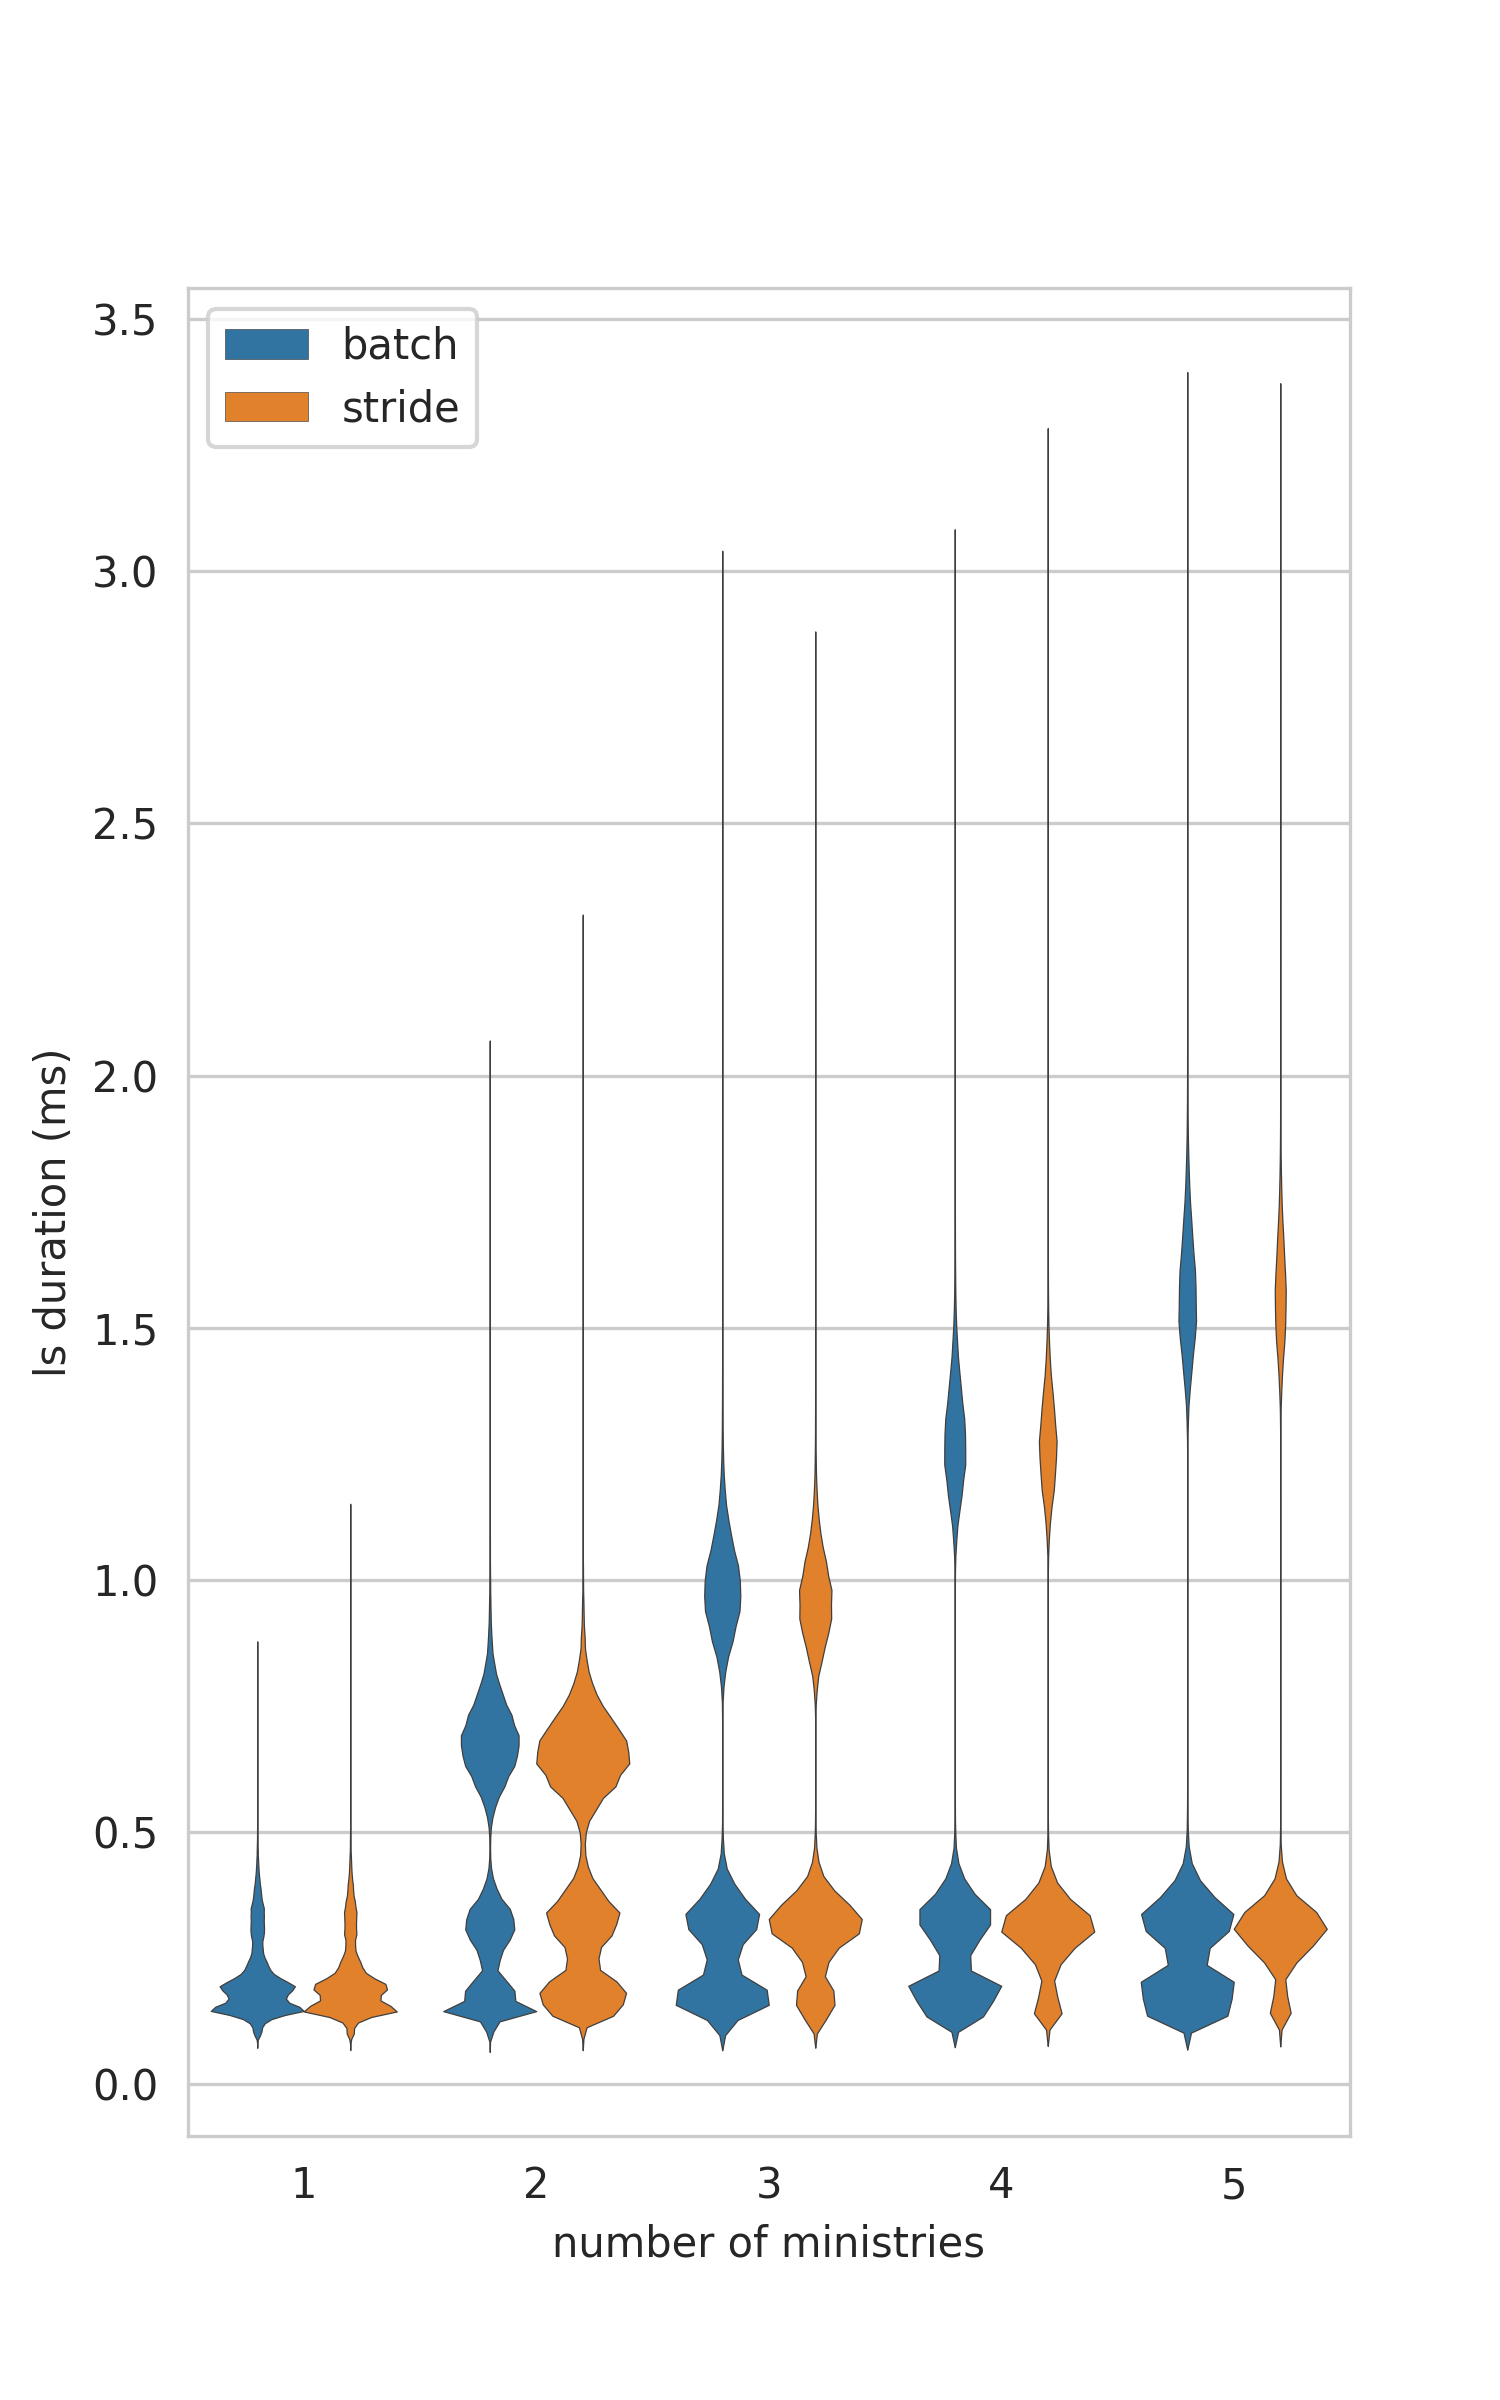
\includegraphics[height=\textheight]{../results/plots/ls_vs_numb_ministries.png}
	\caption{Distribution of list directory duration vs number of ministries for two different request orders. On the Y-axis the time it takes a single request to complete. The X-axis shows the number of ministries the file system is using. The orange distributions are results from runs where $30$ clients ordered their request such that the ministries where accessed one after the other, a stride pattern. The blue distributions show results from runs where $30$ clients used a batch pattern: they first perform all requests for one ministry and then for the next. Outliers further out then $4\sigma$ are not shown}
	\label{fig:ls_vs_ministries}
\end{figure}%

\begin{figure}[htb]
	\centering
	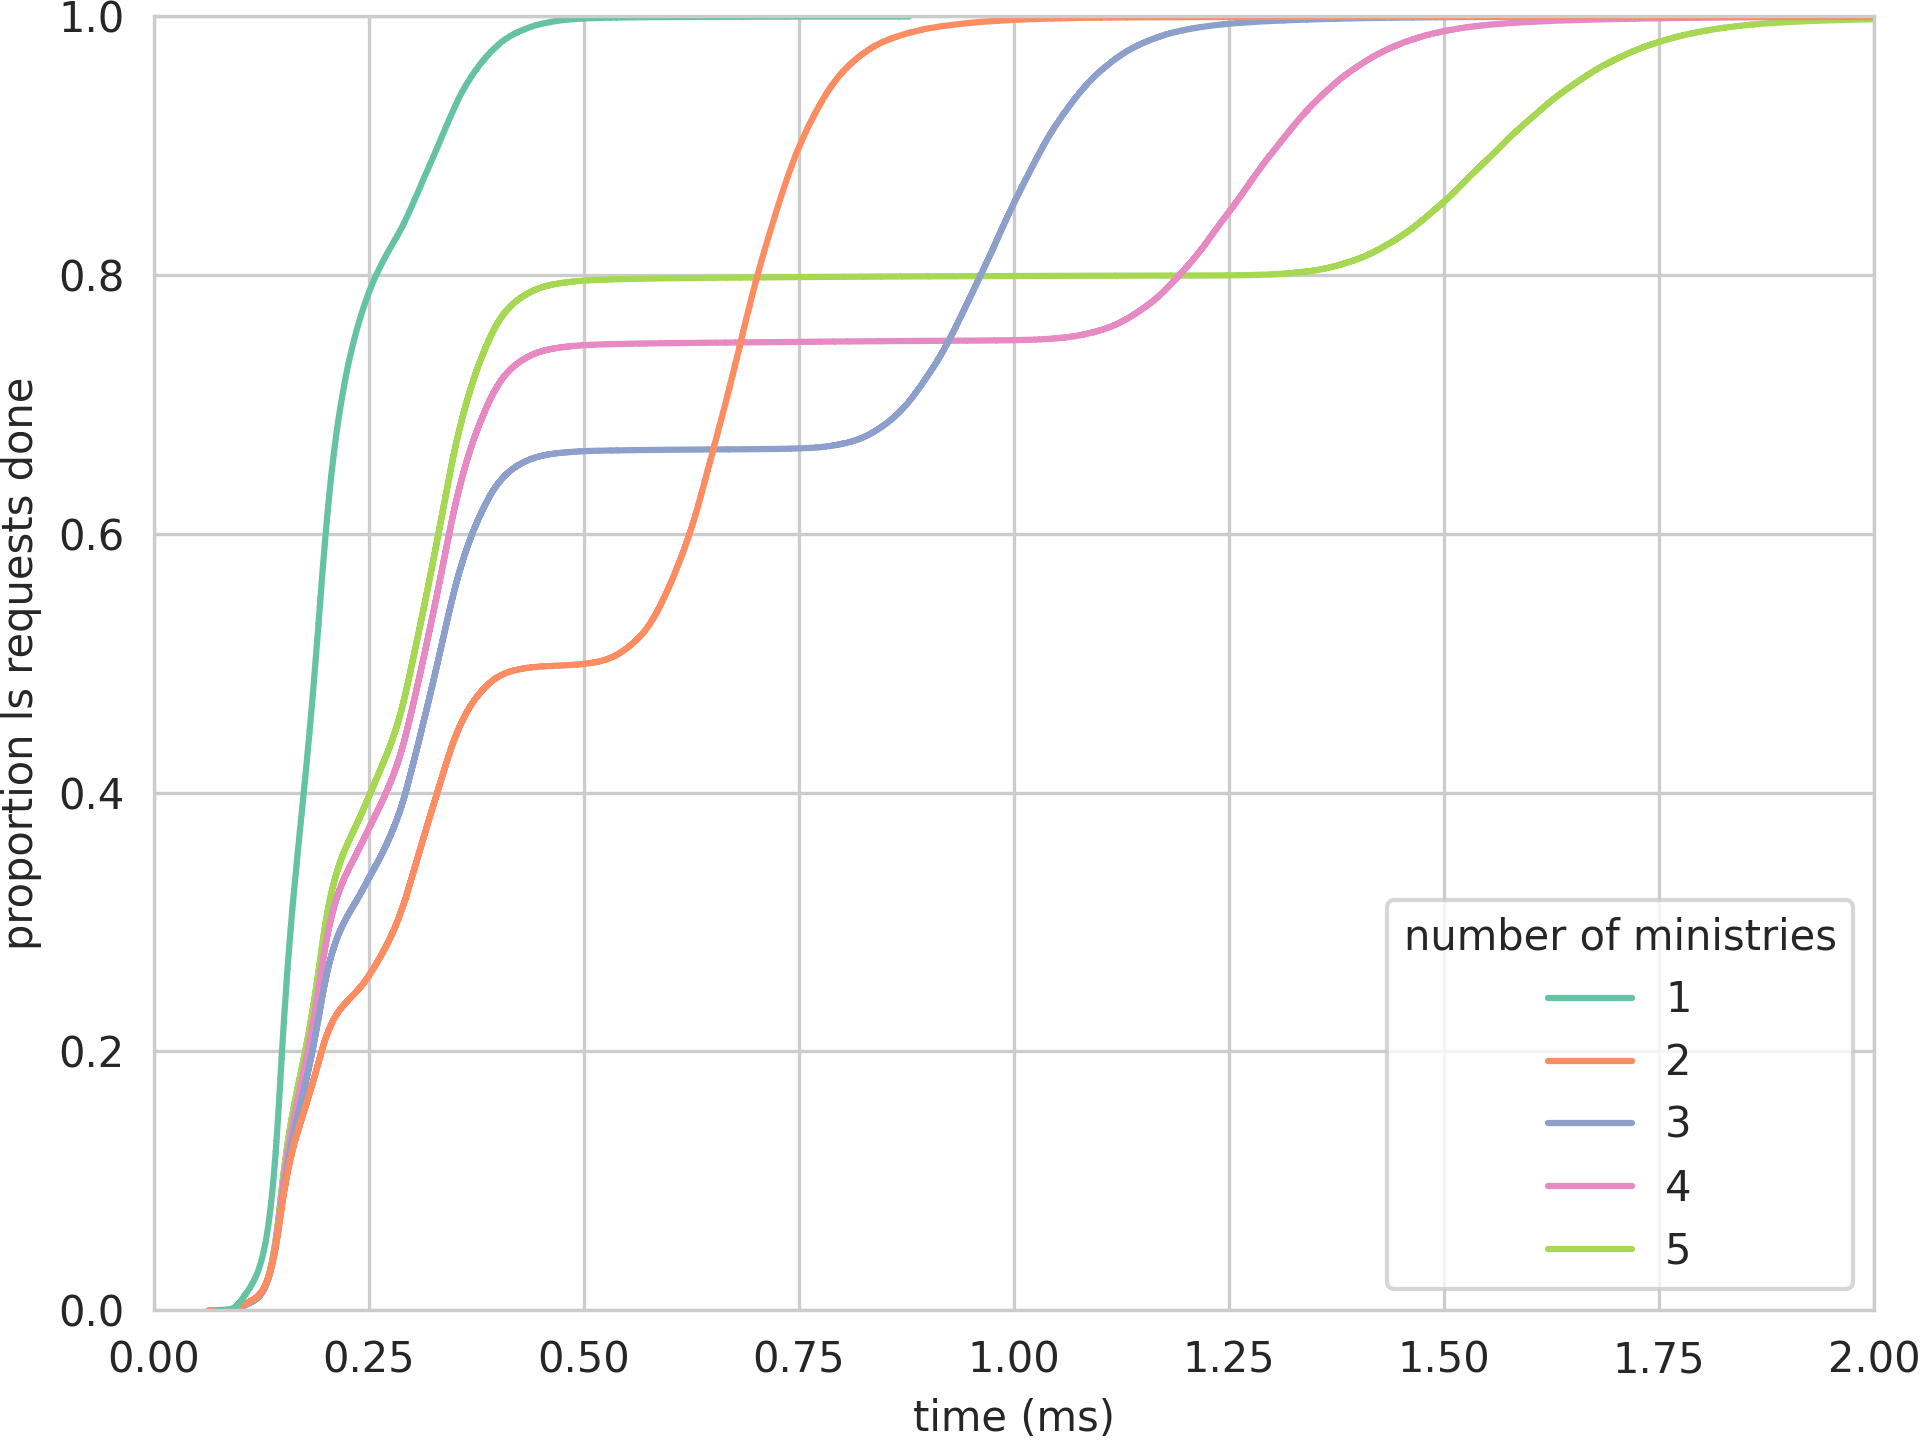
\includegraphics[height=\textheight]{../results/plots/ls_batch.png}
	\caption{\acp{cdf} of clients performing 60 thousand list directory requests for varying amount of ministries. On the Y-axis the proportion of requests completed, at $1.0$ all 60 thousand requests have been answered. The X-axis shows the time until the proportion was reached. The clients batch ordered their requests: they first perform all requests for one ministry and then for the next. The chart goes up to two milliseconds, a tiny fraction of requests take longer then that.}
	\label{fig:ls_cdf}
\end{figure}

\clearpage{}
\subsubsection{Create file}
The second load we try is creating files. To create a file a minister appends a single message to the log making creating files rate limited. Without the rate limit load could increase until the communication with the clerks or the hardware of the nodes becomes the bottleneck.%
%\footnote{That is assuming there are no other bottlenecks. We investigate this by profiling the nodes, see:~\Cref{sec:profile}} % % TODO: re-enable if we have time/it is possible to present the profiling results <04-08-22> 

As adding more ministries could alleviate future bottlenecks it is interesting to see how file create performance scales with the number of ministries even given with the rate limits.

Because of this limit imposed by the implementation we send only 90 create requests. They are sent from 9 clients concurrently. These numbers where empirically determined to maximize the load while keeping the cluster stable enough to complete all the tests.

In \Cref{fig:touch} we see \acp{cdf} for the time it takes to create a file on configurations with a various number of ministries. On the Y-axis the proportion of write requests completed, and the X-axis shows the time in milliseconds. Note the first jump upwards is about 75 milliseconds and all the other jumps are around multiples of 75. The more ministries we use the faster most requests are done. Finally, note the proportion of requests completed jumps up in discrete steps.

\Cref{fig:touch_vs_time} offers another look at the same data. Here we see the time needed for each create as a function of when the request started. Darker tones are requests from tests with more ministries. On the Y-axis we see the time needed to complete the request in seconds while on the (logarithmic) X-axis we see the time a create request was sent. The vertical jumps in the \ac{cdf} (\Cref{fig:touch}) show up as horizontal bands here. For example the lowest horizontal band are requests that took 75 ms which matches the first vertical jump. Note that the gap just after the start of the test.

\begin{figure}[htbp]
	\centering
	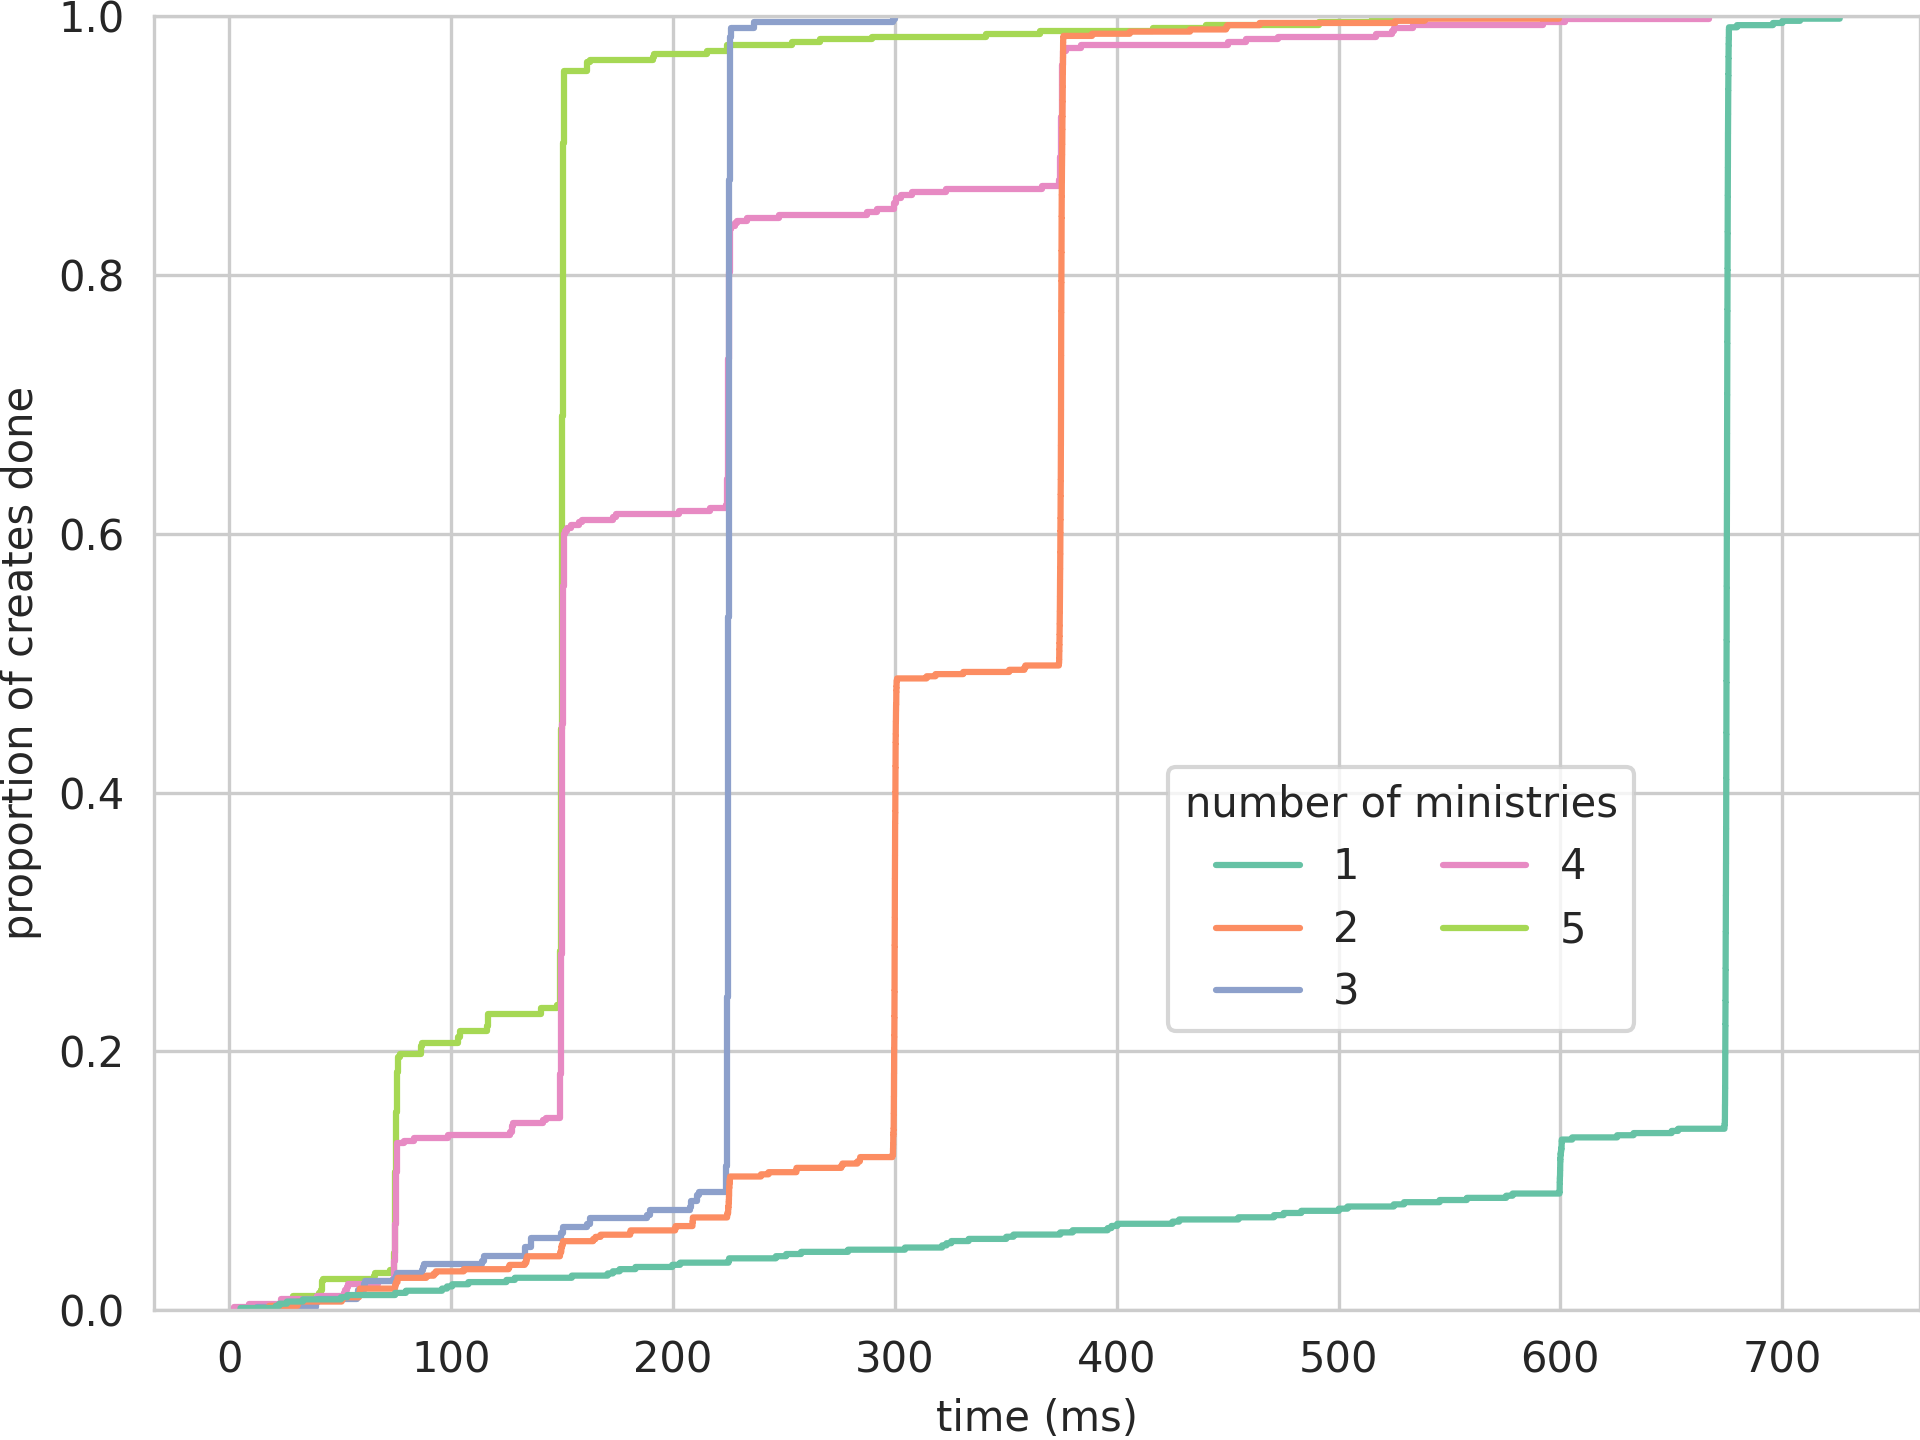
\includegraphics[height=\textheight]{../results/plots/touch.png}
	\caption{\acp{cdf} of clients creating 90 files on clusters with various amount of ministries. On the Y-axis the proportion of files created, at $1.0$ all 90 files have been created. On the X-axis the time in milliseconds until that proportion was reached.}
	\label{fig:touch}
\end{figure}

\begin{figure}[bp]
	\centering
	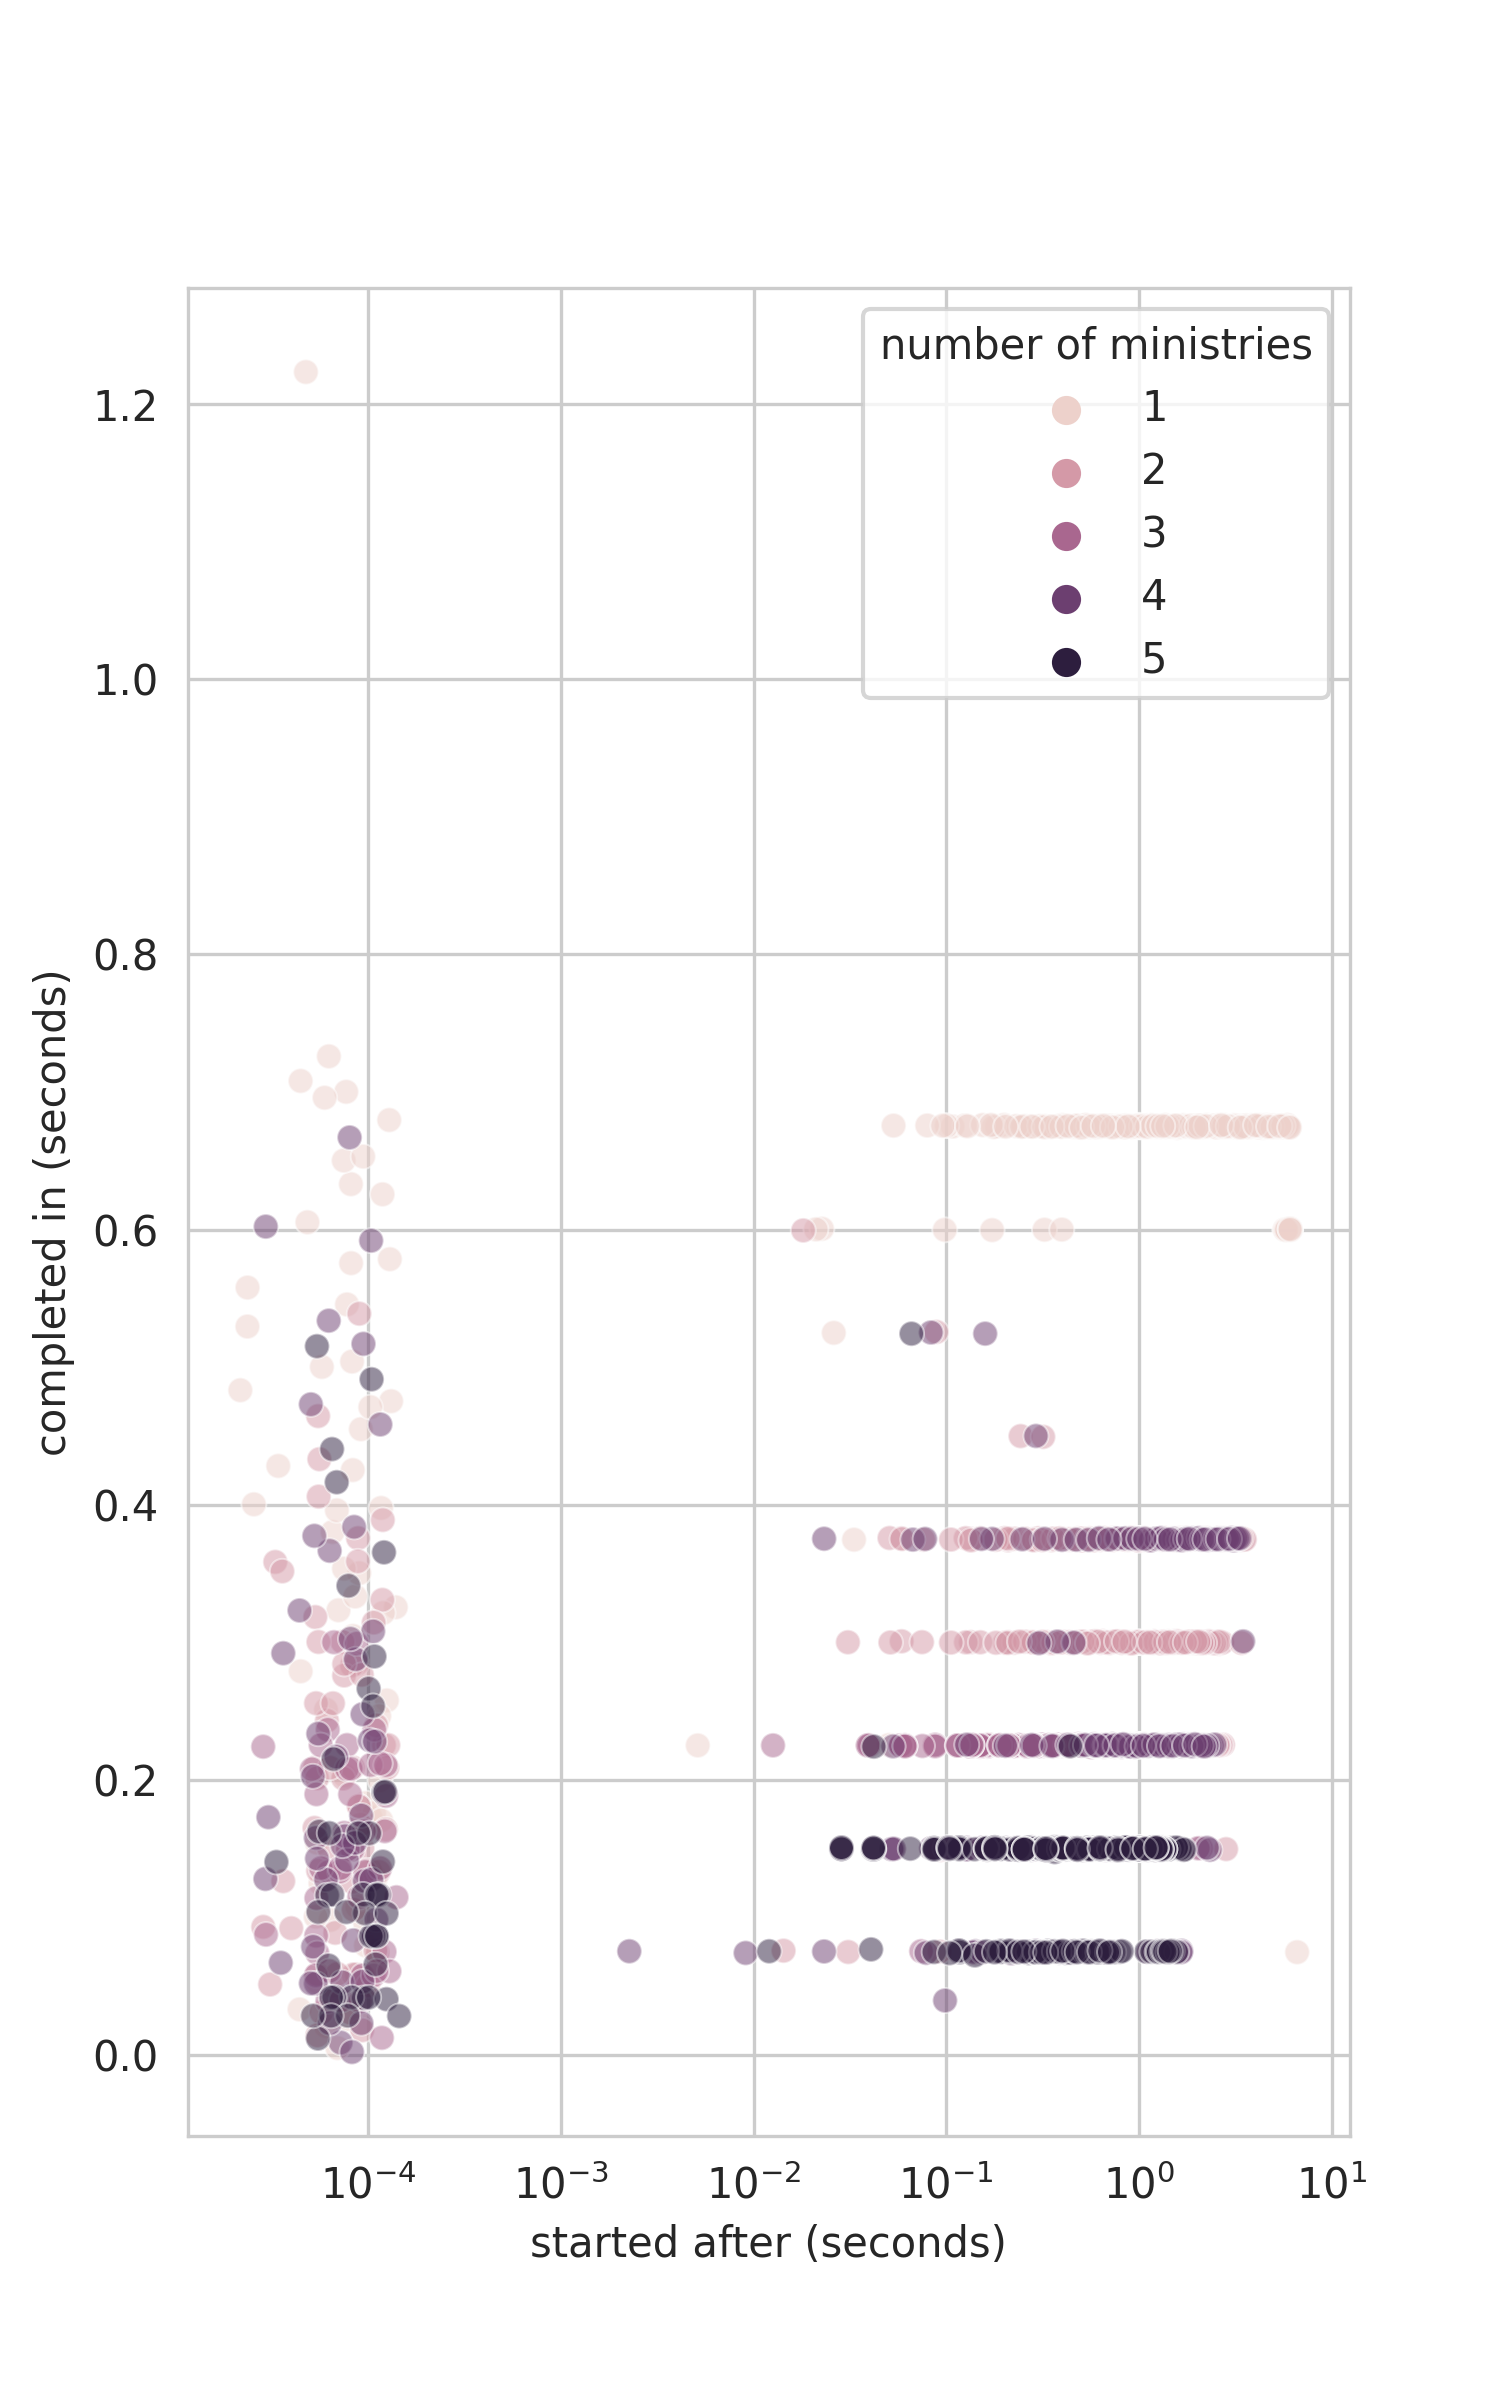
\includegraphics[height=\textheight]{../results/plots/touch_vs_time.png}
	\caption{A logarithmic plot of file create request time vs when the request was started. The same data as in \Cref{fig:touch}. On the Y-axis the time it took a request to complete in seconds while the X-axis shows the point at which the request was started. Darker points are from runs where the system had more ministiers.}
	\label{fig:touch_vs_time}
\end{figure}

\clearpage{}
\subsection{Range based file locking} \label{sec:res_range}
Now we evaluate the contribution of ranged writes compared to writing the entire file. A good use case of ranged file access is writing out one or more rows in a file. In other systems we request exclusive access to the entire file and writing out all the needed rows. Here we can request access to and writ out one row at the time. We expect this second method to be faster when contending with more clients for the same file and with larger files.

Here we compare these methods using two different experiments. In the first experiment we write a single row of a file with 10 rows from multiple clients simultaneously. Each client picks a row at random. In the second experiment we write all rows. Each client uses a random order when writing by row.

We run both experiments for various row size and number of concurrent writers. When varying the row size the number of concurrent writers was fixed at six. While changing the number of writers the row size was kept at 10 \ac{mby}.

Since \name{} has no data plane implementation writing is simulated by sleeping on the client side. We simulate writing at a speed of 200 \ac{mby} per second\footnote{This corresponds to a slow hard drive. That is the best case scenario for writing by row since it increases the ration of time writing versus connecting and locking.}.

In the table below we see the time spend on simulating IO and the average duration for writing one or 10 rows either by locking the whole file or locking by row:
%
\begin{tabular}{lcccccc} \toprule
	& \multicolumn{6}{c}{Row Size (\ac{mby})} \\ \cmidrule(r){2-7}
	                   & 0.1 & 1 & 10 & 20 & 40 & 80 \\ \midrule
	Writing a single row  \\ \cmidrule(r){1-1}
	IO simulation (ms) & 0.5          & 5          & 50          & 100         & 200         & 400 \\
	Lock by row & 411 & 370 & 366 & 444 & 636 & 971\\
	Lock entire file & 62 & 114 & 298 & 618 & 975 & 1644 \\
\smallskip \\
	Writing 10 rows (s)\\ \cmidrule(r){1-1}
	IO simulation & 0.005          & 0.05          & 0.50          & 1         & 2         & 4 \\
	Lock by row & 2.83         & 3.00       & 3.52        & 4.58        & 7.29        & 12.12 \\
	Lock entire file & 0.57         & 0.82       & 1.51        & 2.65        & 4.90        & 9.60 \\ \bottomrule
\end{tabular}
%
In the next two subsections we will look at these results in greater depth.
%
\subsubsection{Writing a single row}
\Cref{fig:single_rowlen} shows the time it takes to write a single row for different row sizes. The Y-axis shows the duration a single write request takes in seconds. Each dot is a single measurement. We see that locking the entire file is slower than locking only the needed row. Note how increasing the row length shrinks the performance gap between these methods. Note furthermore that there are many outliers when locking by row.

\begin{figure}[htbp]
	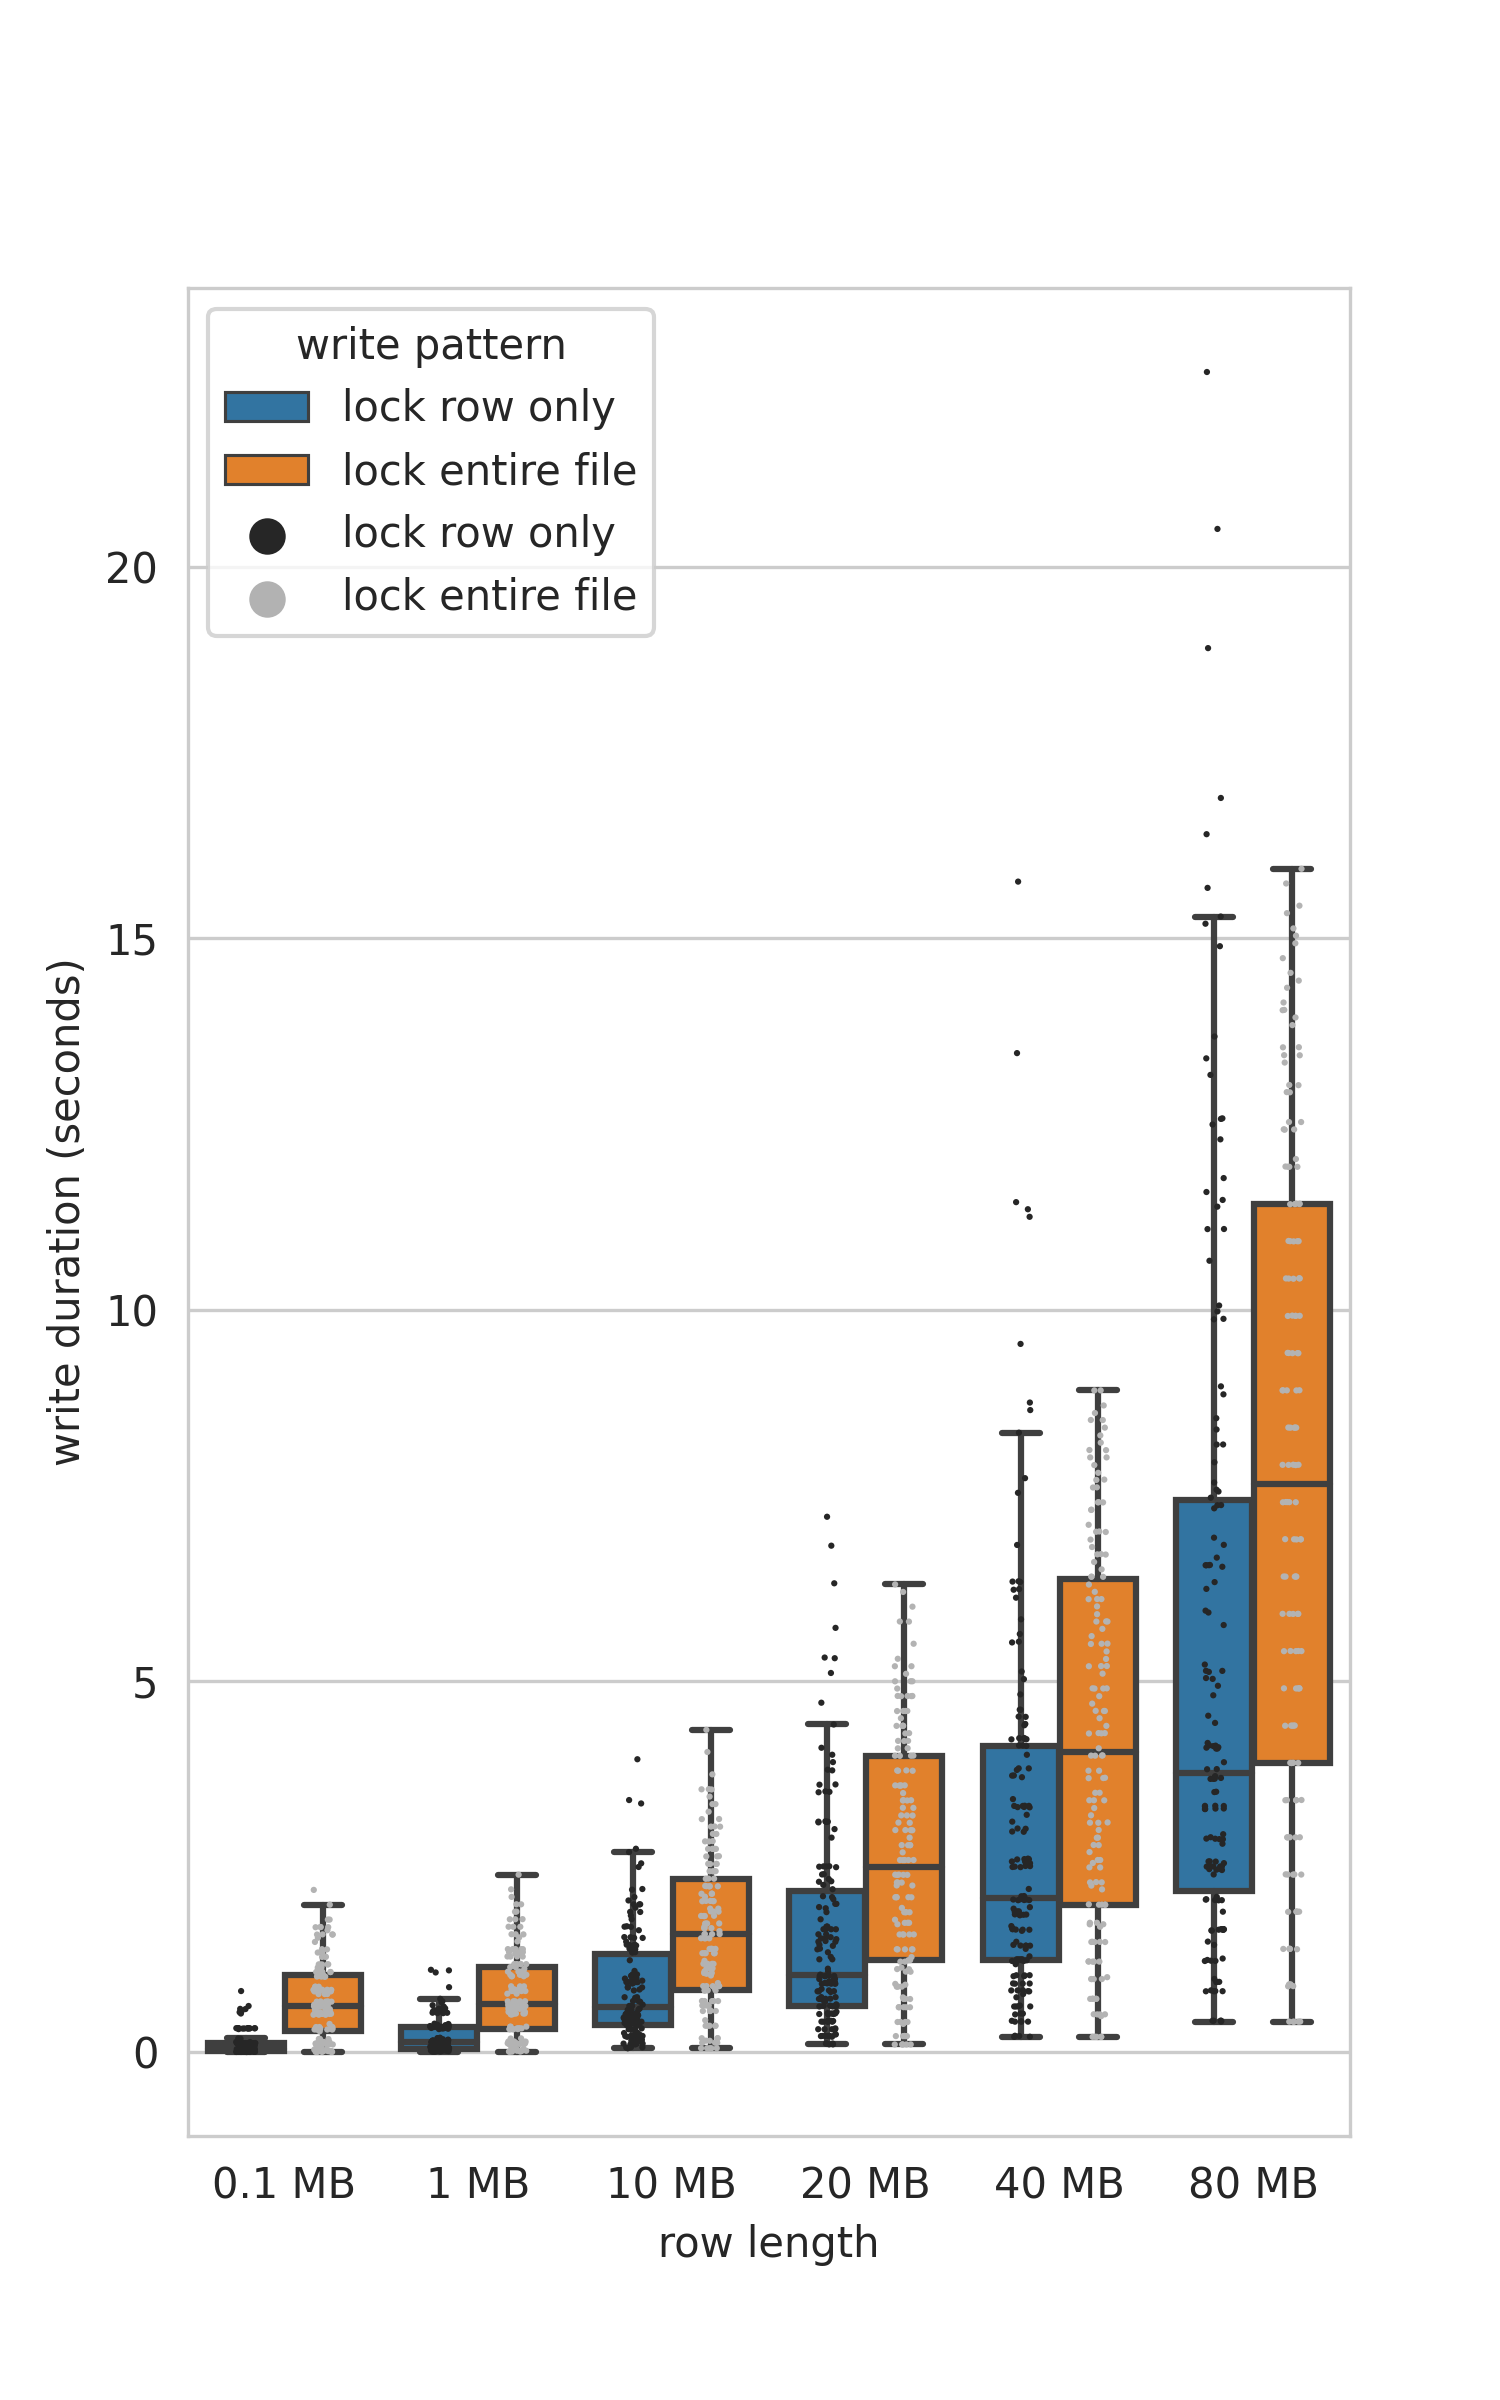
\includegraphics[width=3\textwidth]{../results/plots/single_vs_row_len.png}
	\caption{The time it takes to write a single row given different row sizes. Every dot is a single measurement. On the Y-axis the duration a single write request takes in seconds. On the X-axis the row size in MB. In blue the time needed when only locking the needed row while in orange we see the time needed when locking the entire file.}
	\label{fig:single_rowlen}
\end{figure}
%
In \Cref{fig:single_writers} we see that with more simultaneous writers locking only a single row becomes faster. The Y-axis shows the duration a single write request takes in milliseconds. Note how locking the entire file is faster up to and including 4 writers. This is strange as both methods lock the file once. The results where therefore ran thrice and triple checked.
%
\begin{figure}[htbp]
	\centering
	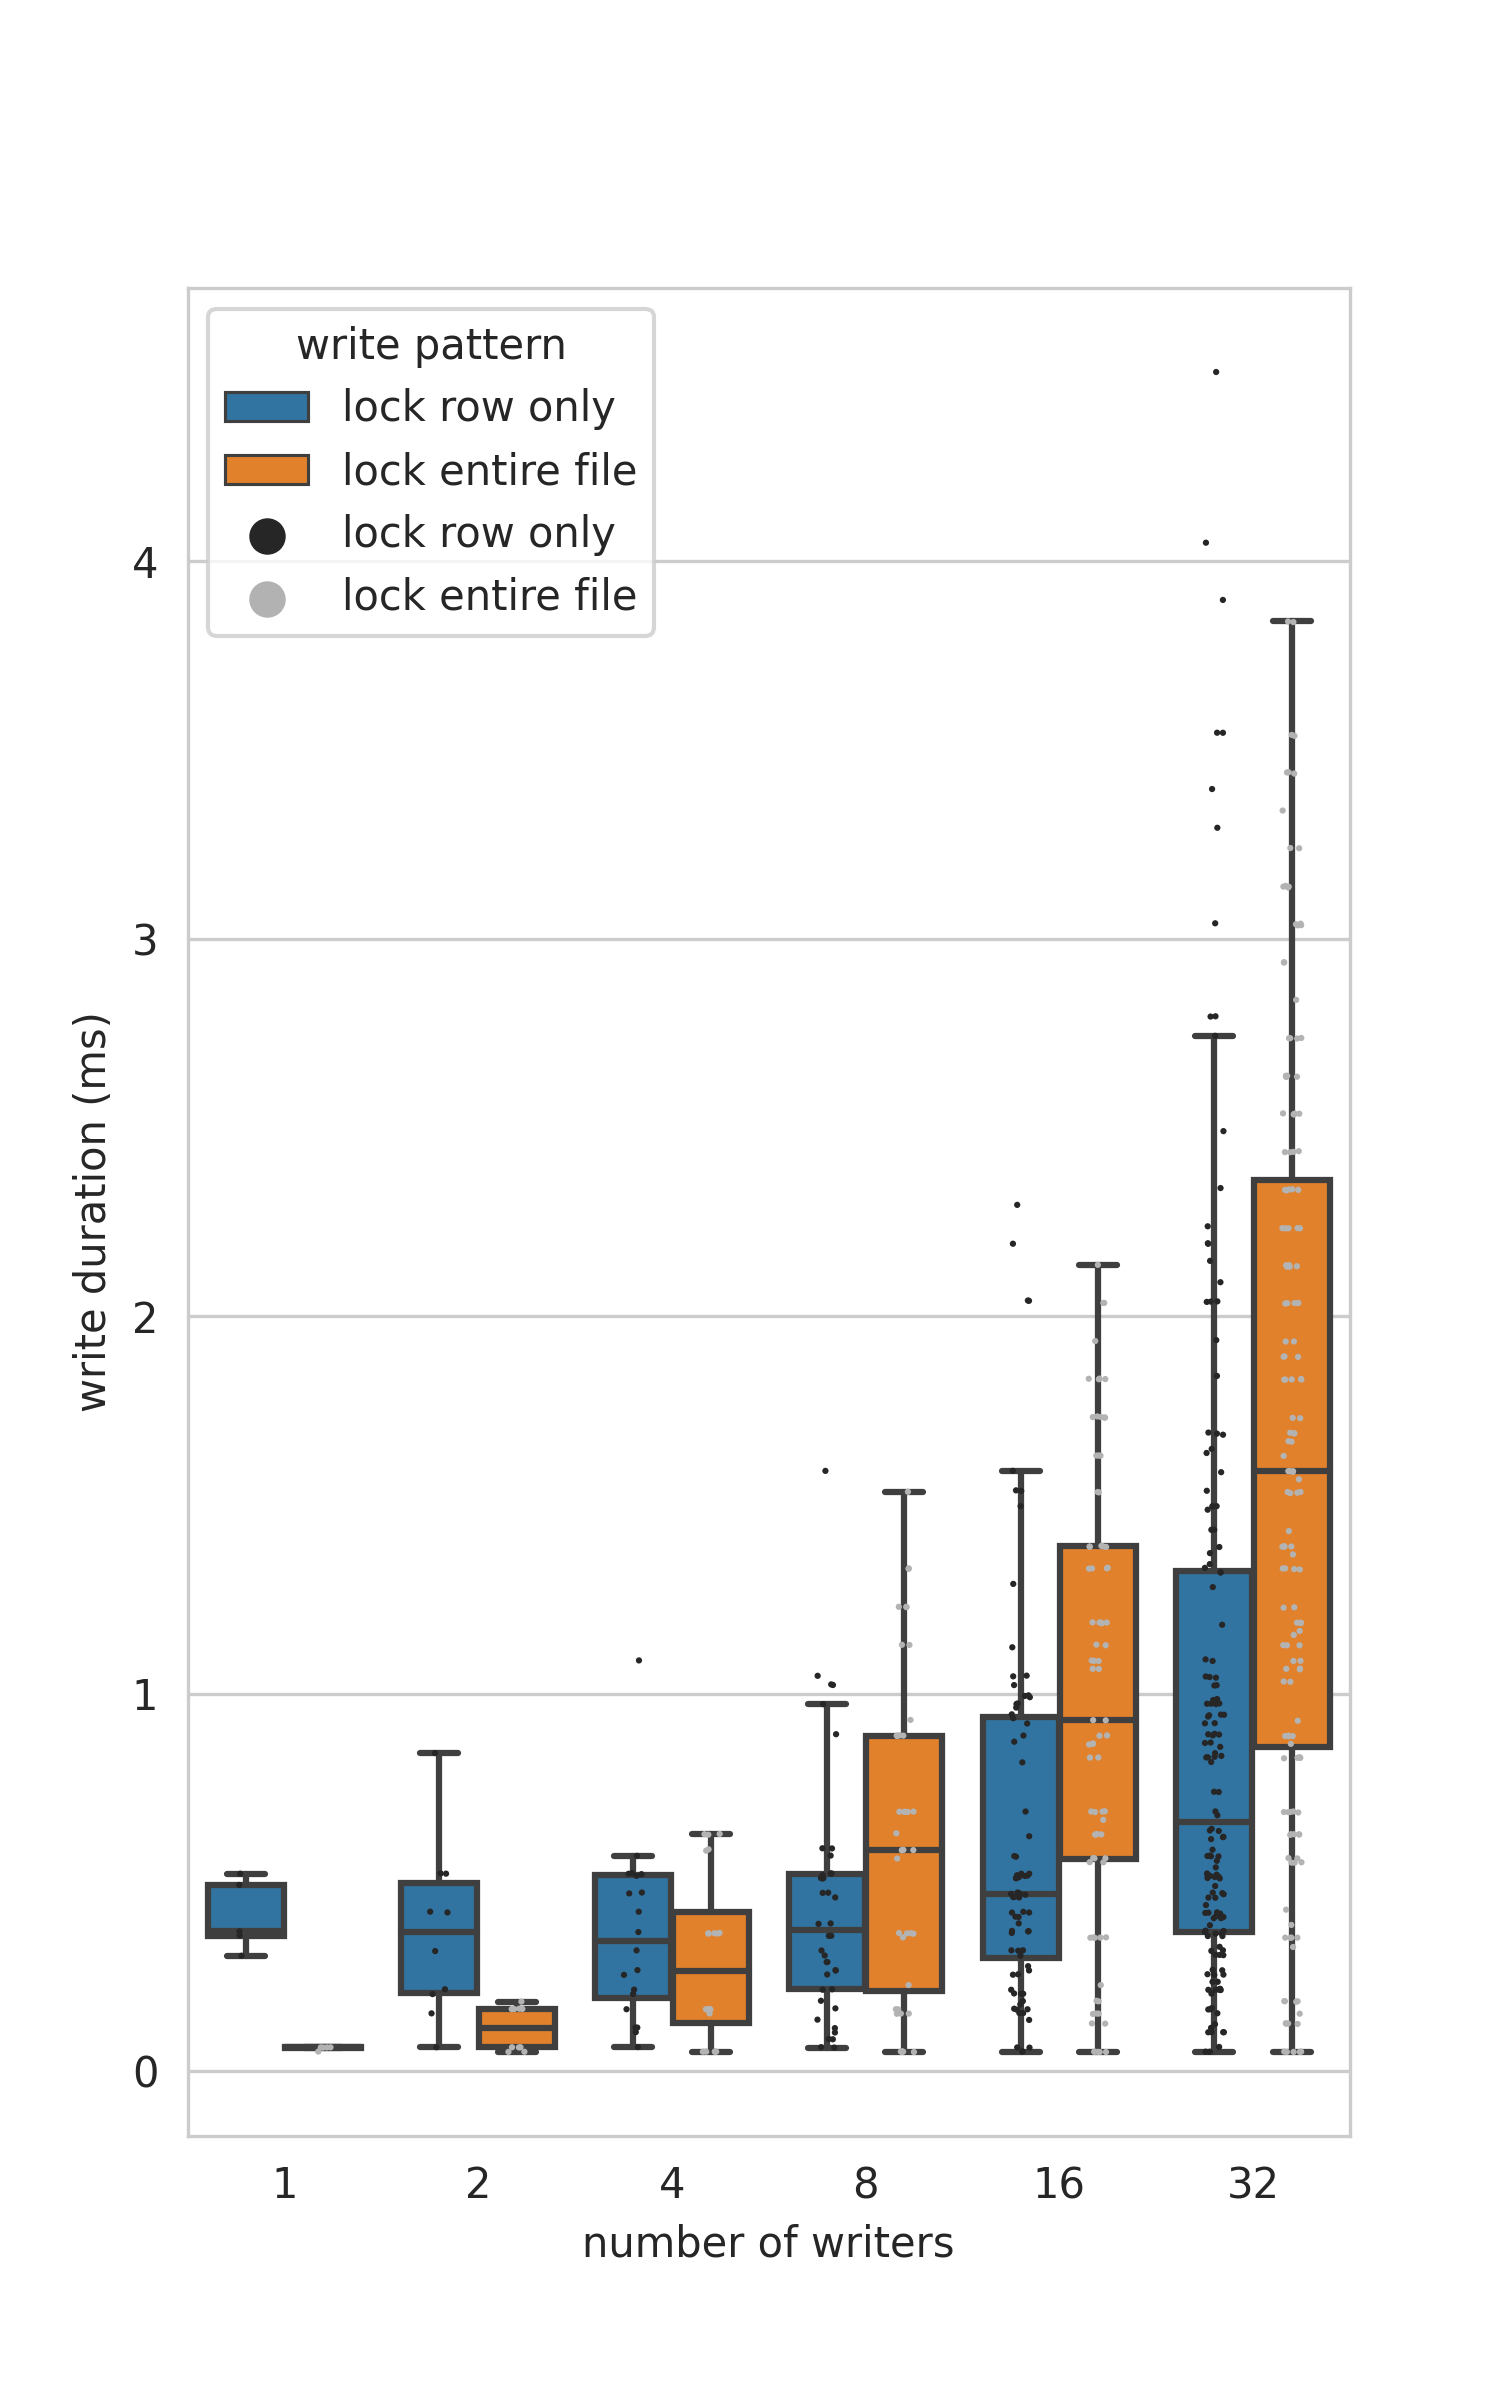
\includegraphics[height=\textheight]{../results/plots/single_vs_writers_both.png}
	\caption{The time it takes to write a single 10 \ac{mby} row given different numbers of writers from 1 to 32. On the Y-axis the duration in milliseconds. The X-axis shows the number of writers, doubling every time. In blue the time needed when only locking the needed row while in orange we see the time needed when locking the entire file.}
	\label{fig:single_writers}
\end{figure}

\clearpage
\subsubsection{Writing the entire file}
In \Cref{fig:rowlen} we look at every individual duration measurement for writing all 10 rows given various row lengths. Again we compare locking by row versus locking the entire file. The logarithmic Y-axis shows the duration in seconds. The X-axis shows various sizes for the rows. As expected larger rows result in longer write durations. Furthermore, we see discrete levels in write duration when writing the entire file and not when writing by row.
%
\begin{figure}[htbp]
	\centering
	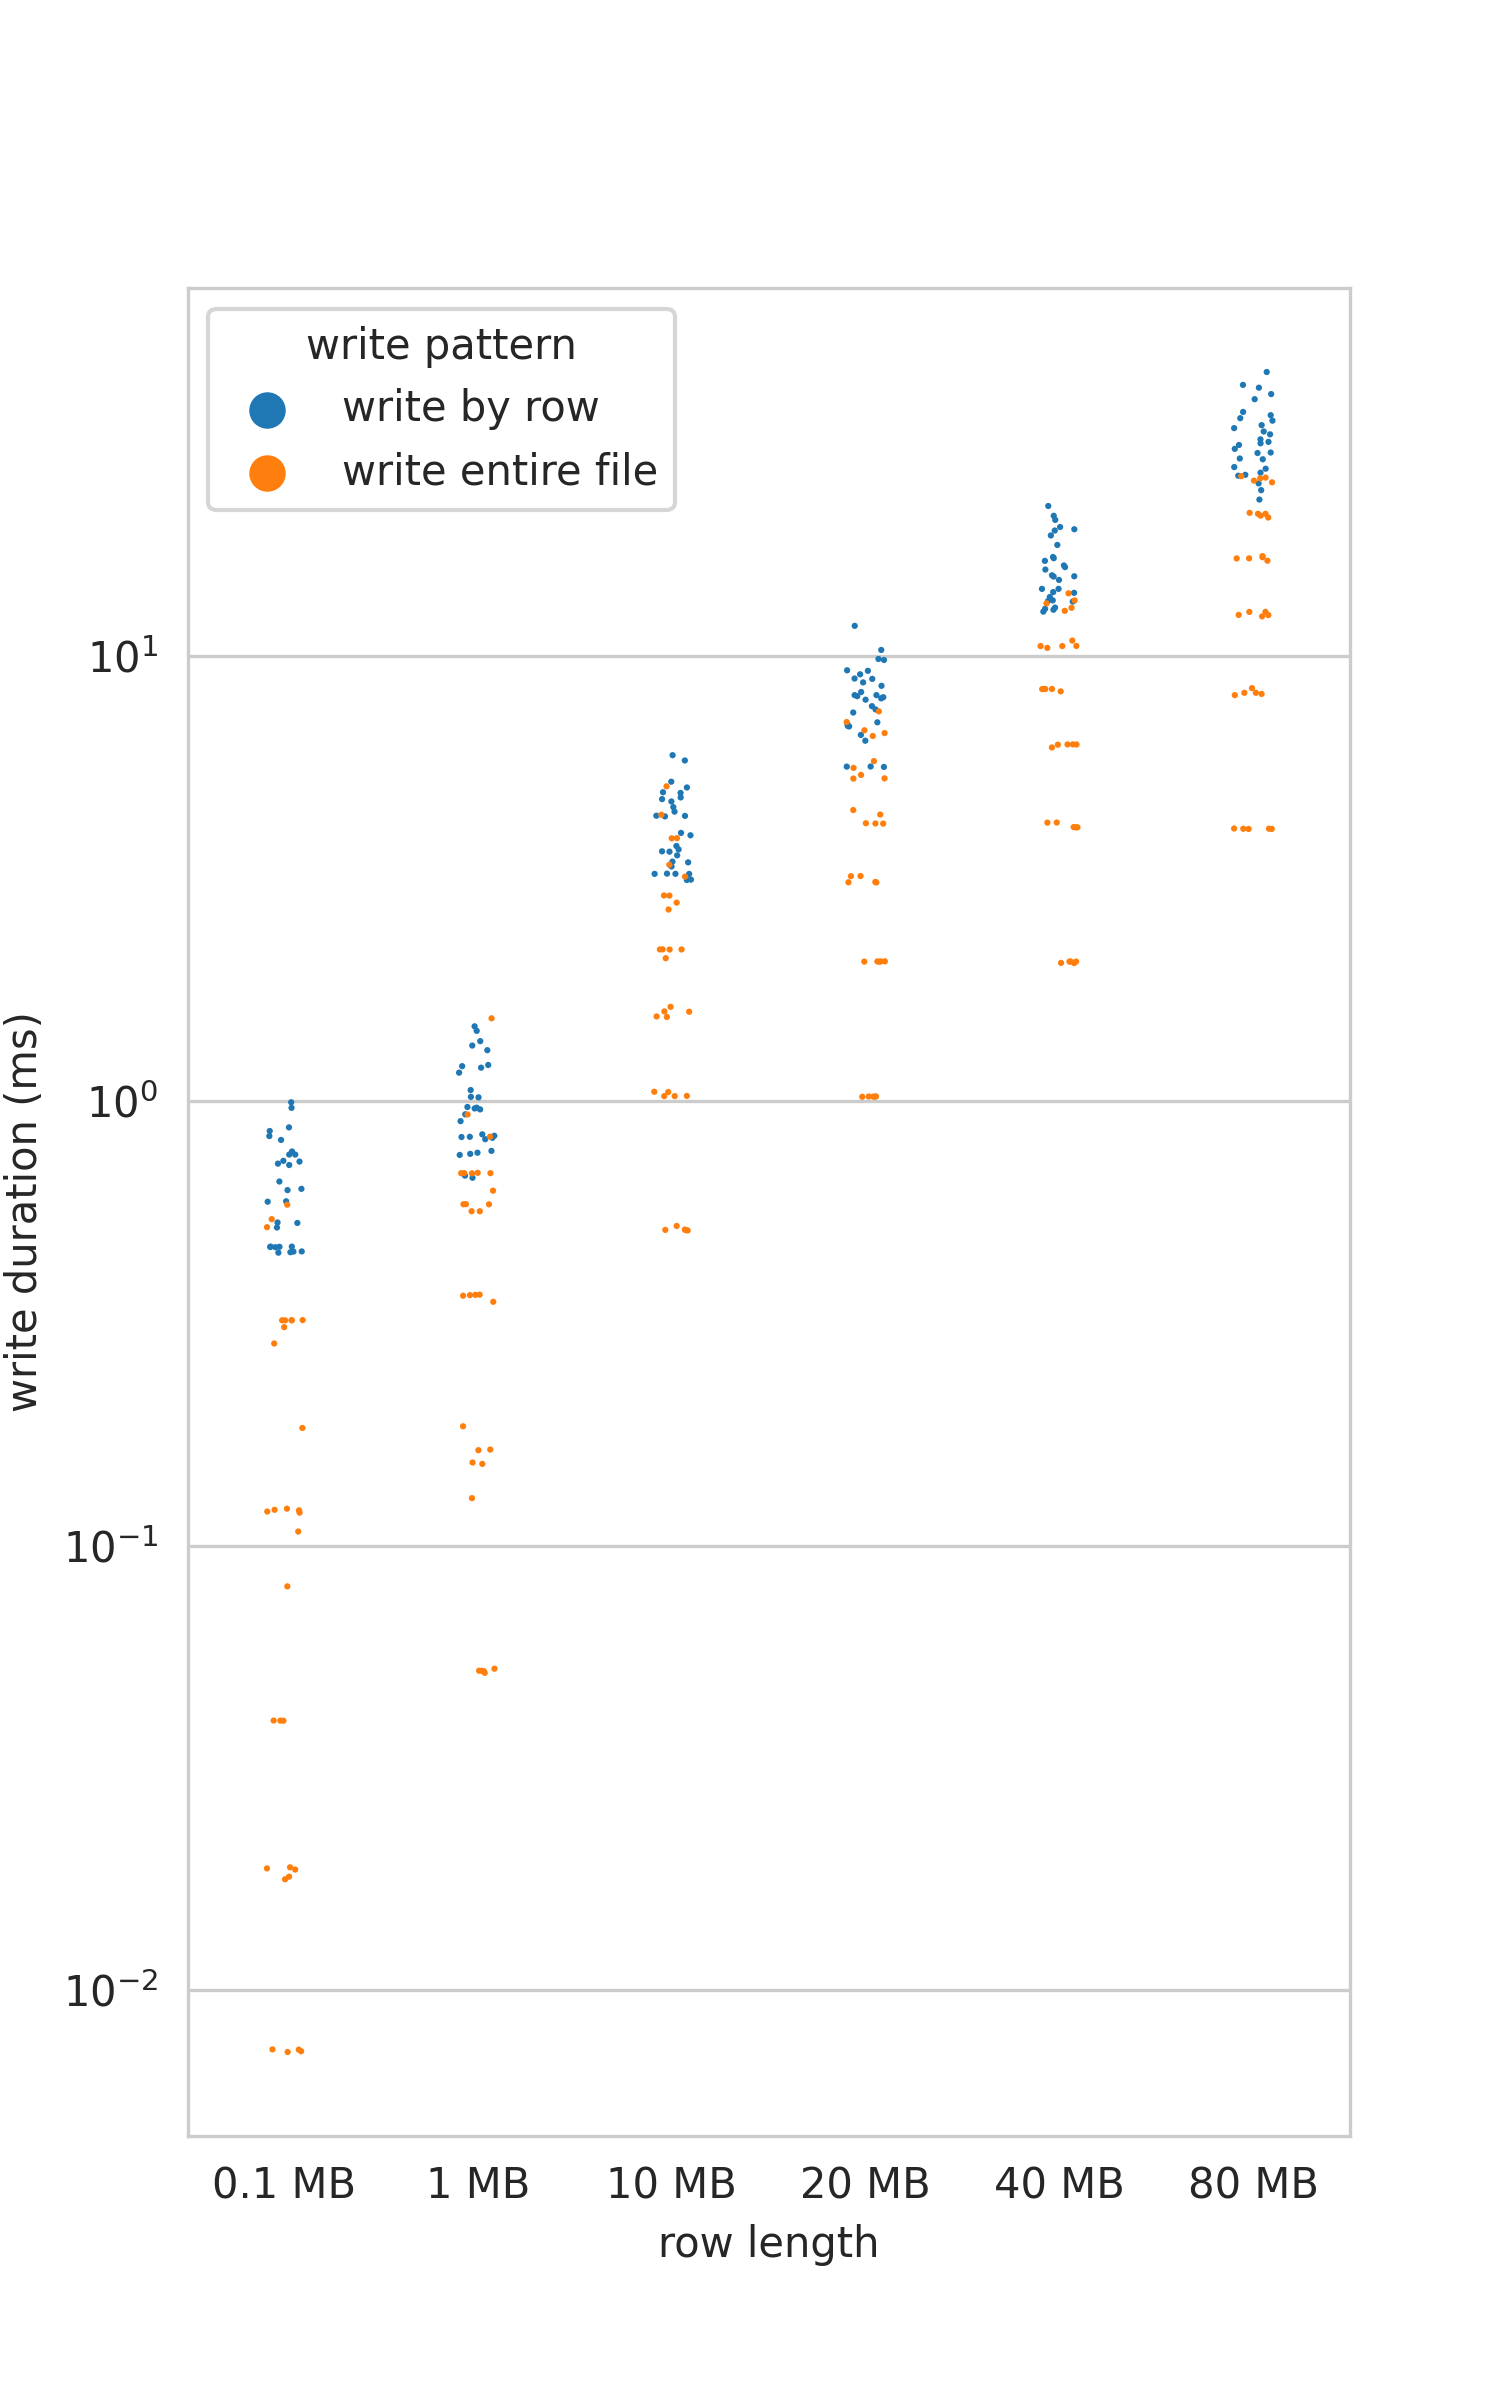
\includegraphics[height=\textheight]{../results/plots/range_vs_row_len.png}
	\caption{The time it takes to write 10 rows for varying row sizes. The blue dots are time measurements when only locking the needed row, locking in total ten times to write all rows. In orange the duration when locking the entire file and writing all rows at once.}
	\label{fig:rowlen}
\end{figure}%

\Cref{fig:writers} again shows the duration it takes to write all the rows this time for varying number of writers, comparing locking by row versus locking the entire file. The Y-axis shows the time it takes to write all 10 rows. Note how writing by row takes significantly longer with the gap closing when the number of writers increases. Also note the uniform distribution between the fastest and slowest time when locking the entire file (orange).
%
\begin{figure}[htbp]
	\centering
	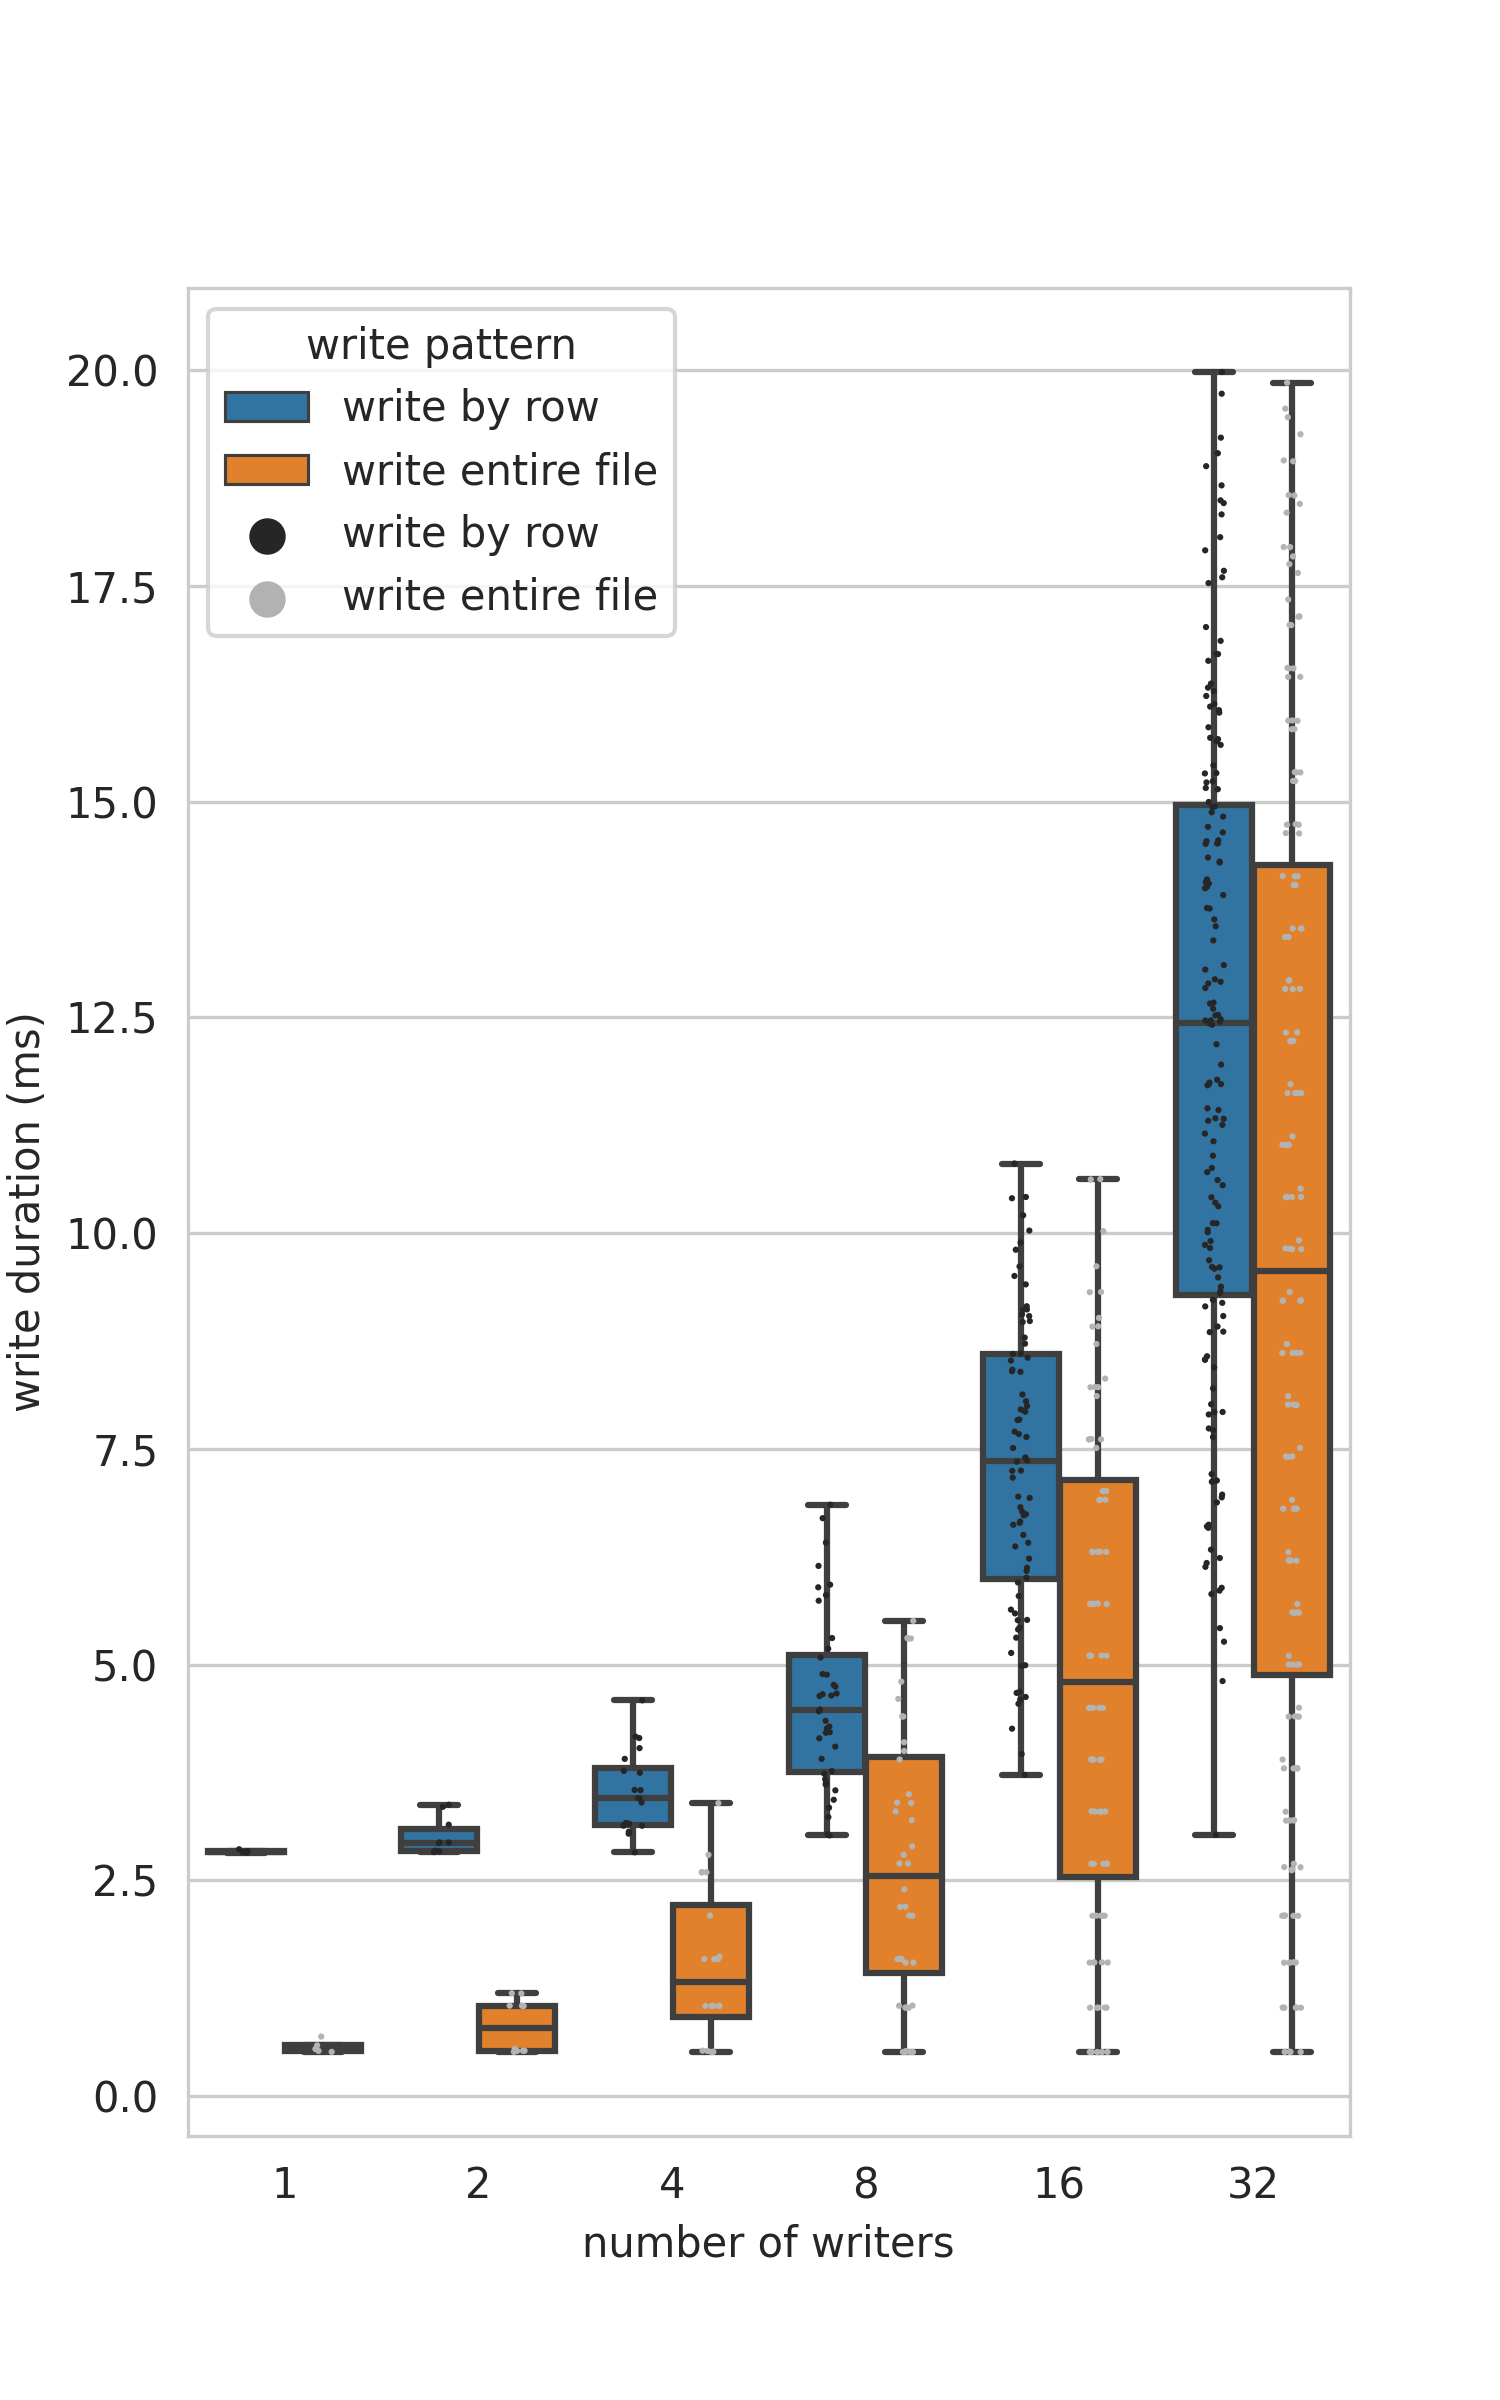
\includegraphics[height=\textheight]{../results/plots/range_vs_writers_both.png}
	\caption{The time it takes to write ten rows with between one and 32 concurrent writers. On the logarithmic Y-axis the duration in milliseconds. In blue the duration when only locking the needed row, locking in total ten times to write all rows. In orange the result when locking the entire file and writing all rows at once.}
	\label{fig:writers}
\end{figure}

\clearpage

%\subsection{Profiling} \label{sec:profile}
% for now we are not doing this (time limitations)


\section{Discussion} \label{sec:discussion}
In the previous section we presented the performance of \name{}. We focussed on its two distinguishing features: the \textit{ministry architecture} and its \textit{ranged based file locking}. Another important characteristic of any system is its complexity. The main contribution of the \raft{} consensus algorithm is a more understandable solution that is therefore easier to implement. We begin by discussing the complexity of \name{} then we discuss the performance implications of the \textit{ministry architecture} before we finish discussing \raft{ranged based file locking}.
%
\subsection{Complexity}
Raft is an understandable consensus algorithm. Here we have extended it to get \textit{Group Raft} which provides greater scalability. This extended algorithm had two problems. These where both solved by re-using the Raft concept of terms. No new variables where added to the algorithm nor did we add new routines. It is still quite simple. 

\Name{} clerks need to know if their log is running behind. For this we added Perishable Log entries to \textit{Group Raft}. These use log entry arrival time, the groups leaders commit index and the heartbeat duration to determine if a log entry is applied on time. Tracking arrival time is a trivial addition. All other variables where already available making perishable a simple addition.

As leases did not need to survive system crashes and reboots we did not use Raft but designed our own algorithm for non-persistent consistency. This enables \name{} to reach higher read and write performance. Even non-persistent consistency is still a hard problem, therefore this algorithm makes \name{}'s implementation significantly more complex. In \Cref{sec:impl_leases} we saw there are four known problems with this algorithm. While most have solutions solving these will further increase the now already high degree of complexity.
%
\subsection{Ministry architecture}
\paragraph{Design Faults}
During testing, we realized there is a fault in the current design. The president is responsible for detecting nodes that go down. However, if the president can reach a clerk and its minister that does not guarantee that the clerk and minister can reach each other. We can address this by nodes informing the president when they can not reach one of their assigned nodes.
\paragraph{List Directory}
We saw the fastest response from a \name{} configuration using only a single ministry. As soon as we start using multiple latency increases. Adding more ministries increases average performance. Clients start without knowledge of the configuration, they are designed to initially connect to a random node. It is therefore logical that we see an increased in latency with more ministries: given twice as many ministries the chance to connect to the right node on the first try halves. 

As expected the request order \textit{batch} order is faster than \textit{stride}. We would however expect there to be a larger difference. We did not expect the difference to get more pronounced as the number of ministries increases. It could be that it takes the client longer to re-establish its connection when the connection has been out longer. This requires study of the clients' performance and implementation.

The tail latencies become longer as we increase the number of ministries. This is unexpected. Requests should arrive at the right ministry after at most one redirect. The number of requests that need a redirect should increase as the number of ministries increases however those redirects should take the same amount of time. An explanation could be that the higher number of redirects overloads the redirect system leading to longer response times for those queries.
%
\paragraph{Create file} 
Mean file creation time decreases almost linearly with the number of ministries. This should hold true even after the Raft implementation has been improved. Most file creation complete in a multiple of 75ms. This corresponds to the heartbeat duration used for Raft which imposes a rate limits on log modifications in this implementation. 

Up to 5\% of writes are completed in less time. At least a heartbeat period must pass before a new log entry can be appended. Only after appending the log entry does the minister inform the client the creation is done. Further study is required to explain these results.
%
\subsection{Ranged based file locking}
\paragraph{Writing a single row}
Locking only the needed data when writing to a file gives a dramatic increase in performance. This is in line with our expectations as the chance of lock contention decreases given less overlap in lock regions. Given larger files the difference in performance between the methods decreases as the time spend on (simulated) IO starts to dominate the time spend on locking. There are some far outliers that only appear when using row locking at the same time the variance of row locking is lower. We have no explanation for this, and it should be studied further starting with the behavior of the client.

In this experiment both methods lock the file once and both locks should succeed in the same time given the files start unlocked. The only difference is the range of the lock that is acquired. Locking the entire file is however much faster. This even holds with a single writer in which case there can be no contention. With only a single writer both methods should therefore do exactly the same and have the same results. Only when using more than four simultaneous writers do we see locking the smaller range becoming faster. Given these results, especially the results when using a single writer, there is a fault in either the test or the lease system.
%
\paragraph{Writing the entire file}
The lower lock contention when locking by row does not make up for the overhead of extra lock operations when locking ten times. Even when using very large files with rows of 80 \ac{mby} locking the entire file is significantly faster. The gap does seem to close as row size increases. There is a uniform distribution of results when locking the entire file. This distribution highlights how each write can only be started after the previous completes. The width of the distribution comes from the five separate runs that are presented.


\section{Future work} \label{sec:fut}
Although we did not succeed in building a performant system we found a number of interesting avenues for improvement. These fall into three categories: dynamic scaling, more efficient Group Raft and ranged leases.

\subsection{Dynamic scaling}
The \name design includes load balancing through shaping the systems' configuration to the current load. Using subtree partitioning to spread directories across more or less ministries. In \cref{sec:tradeoff} we discussed the trade-off between read or write performance. This trade-off could be transformed into constrained optimization problem. It would be interesting to have \name{} keep an optimal configuration by continuously solving this problem. To allow users to specify to what degree each file should be replicated the replication factor can be added as additional constraint.

\subsection{Consensus}
The \textit{Group Raft} implementation is very inefficient because it sends only one log entry at the time at fixed intervals. An efficient implementation will make it possible to directly compare \name{} with existing distributed FS. We expect a dramatic speedup by batching Raft log messages and sending them on demand. Since modifications to different directories can never impact each other we can use a combination of \textit{ParallelRaft}~\cite{polarfs} and \textit{Group Raft}.

Currently, any node will start an election if it misses a heartbeat. Ministers can, and sometimes are elected as president. The loss of the minister causes its ex-ministry to pause metadata changes and file writes while a clerk is promoted and a replacement clerk assigned. Banning ministers for taking part in elections and preferring idle nodes to clerks will prevent such pauses.

One reason for re-elections is newly elected presidents taking too long to establishing connections and start emitting heartbeats. A better implementation would re-use the connections a candidate established asking for votes when it becomes president.

As groups only communicate with their members, clients and the president. Communication with the president does not require low latency nor high throughput. This could make \textit{Group Raft} really useful for geo-distributed systems, that is systems consisting of clusters in different locations. As long as the members of each group are kept to the same location normal performance should not decrease.

\subsection{Leases}
Every write triggers a request to all the clerks to stop giving out read leases. This is inefficient for files experiencing mostly writes or for consecutive small writes. Ministers should keep files locked when the files are experiencing high write load. Ranged writes would then become suitable for concurrently writing a file from multiple clients using small non overlapping chunks.

Ranged locking should enable better performance in workloads with lots of reading and writing. It would be interesting to have this difference quantified.

The locking implementation does not batch requests. We suspect batching will significantly increase throughput under load.


\clearpage
\appendix
\section{Introduction to Async} \label{app:async}
\textit{Async} is a syntactic language feature that allows for easy construction of asynchronous non-blocking functions. \textit{Asynchronous} programming lets us write concurrent, not parallel, tasks while looking awfully similar to normal blocking programming. It is a good alternative to \textit{event-driven} programming which tends to be verbose and hard to follow. All \textsc{Async} systems are build around special function that do not return a value but rather a \textit{promise} of a \textit{future} value. When we need the value we tell the program not to continue until the promise is fulfilled. Let's look at the example of downloading 2 files:

\begin{lstlisting}[language=rust, style=boxed, tabsize=2]
async fn get_two_sites_async() {
	// Create two different "futures" which, when run to 
	// completion, will asynchronously download the web pages.
	let future_one = download_async("https://www.foo.com");
	let future_two = download_async("https://www.bar.com");

	// Run both futures to completion at the same time.
	let futures_joined = join!(future_one, future_two);
	// Run them to completion returning their return values
	let (foo, bar) = futures_joined.await;
	some_function_using(foo,bar);
}
\end{lstlisting}

Notice the \texttt{async} keyword in front of the function definition, it means the function will return a promise to complete in the future. The \texttt{join!} statement on line 8 combines the two promises for a future answer to a single promise for two answers. In line 10 we await or 'block' the program until \texttt{futures\_joined} turns into two value. Those can then be used in normal and async functions.

The caller of our \texttt{async} \textit{get\_two\_sites\_async} function will need to be another async function that can await \textit{get\_two\_sites\_async}, or it can be an executor. An executor allows a normal function to await async functions.

Let's go through our example again explaining how this mechanism could work. The syntax and workings of async differ a lot here we will look at the language \textit{Rust}. In rust these promises for a future value are called futures. Until the program reaches line 10 no work on downloading the example sites is done. This is not a problem as the results, \textit{foo} and \textit{bar}, are not used before line 11. The runtime will start out working on downloading \texttt{www.foo.com}, probably by sending out a DNS request. As soon as the DNS request has been sent we need to wait for the answer, we need it to know to which IP to connect to download the site. At this point the runtime will instead of waiting start work on downloading bar where it will run into the same problem. If by now we have received an answer on our DNS request for \textit{www.foo.com} the runtime will continue its work on downloading foo. If not the runtime might continue on some other future available to it that can do work at this point.

\printbibliography

\end{document}

\pagestyle{scrheadings} % Show chapter titles as headings
\cleardoublepage % Avoids problems with pdfbookmark
